% Options for packages loaded elsewhere
\PassOptionsToPackage{unicode}{hyperref}
\PassOptionsToPackage{hyphens}{url}
%
\documentclass[
]{article}
\usepackage{lmodern}
\usepackage{amssymb,amsmath}
\usepackage{ifxetex,ifluatex}
\ifnum 0\ifxetex 1\fi\ifluatex 1\fi=0 % if pdftex
  \usepackage[T1]{fontenc}
  \usepackage[utf8]{inputenc}
  \usepackage{textcomp} % provide euro and other symbols
\else % if luatex or xetex
  \usepackage{unicode-math}
  \defaultfontfeatures{Scale=MatchLowercase}
  \defaultfontfeatures[\rmfamily]{Ligatures=TeX,Scale=1}
\fi
% Use upquote if available, for straight quotes in verbatim environments
\IfFileExists{upquote.sty}{\usepackage{upquote}}{}
\IfFileExists{microtype.sty}{% use microtype if available
  \usepackage[]{microtype}
  \UseMicrotypeSet[protrusion]{basicmath} % disable protrusion for tt fonts
}{}
\makeatletter
\@ifundefined{KOMAClassName}{% if non-KOMA class
  \IfFileExists{parskip.sty}{%
    \usepackage{parskip}
  }{% else
    \setlength{\parindent}{0pt}
    \setlength{\parskip}{6pt plus 2pt minus 1pt}}
}{% if KOMA class
  \KOMAoptions{parskip=half}}
\makeatother
\usepackage{xcolor}
\IfFileExists{xurl.sty}{\usepackage{xurl}}{} % add URL line breaks if available
\IfFileExists{bookmark.sty}{\usepackage{bookmark}}{\usepackage{hyperref}}
\hypersetup{
  pdftitle={Raport\_finalny},
  hidelinks,
  pdfcreator={LaTeX via pandoc}}
\urlstyle{same} % disable monospaced font for URLs
\usepackage[margin=1in]{geometry}
\usepackage{color}
\usepackage{fancyvrb}
\newcommand{\VerbBar}{|}
\newcommand{\VERB}{\Verb[commandchars=\\\{\}]}
\DefineVerbatimEnvironment{Highlighting}{Verbatim}{commandchars=\\\{\}}
% Add ',fontsize=\small' for more characters per line
\usepackage{framed}
\definecolor{shadecolor}{RGB}{248,248,248}
\newenvironment{Shaded}{\begin{snugshade}}{\end{snugshade}}
\newcommand{\AlertTok}[1]{\textcolor[rgb]{0.94,0.16,0.16}{#1}}
\newcommand{\AnnotationTok}[1]{\textcolor[rgb]{0.56,0.35,0.01}{\textbf{\textit{#1}}}}
\newcommand{\AttributeTok}[1]{\textcolor[rgb]{0.77,0.63,0.00}{#1}}
\newcommand{\BaseNTok}[1]{\textcolor[rgb]{0.00,0.00,0.81}{#1}}
\newcommand{\BuiltInTok}[1]{#1}
\newcommand{\CharTok}[1]{\textcolor[rgb]{0.31,0.60,0.02}{#1}}
\newcommand{\CommentTok}[1]{\textcolor[rgb]{0.56,0.35,0.01}{\textit{#1}}}
\newcommand{\CommentVarTok}[1]{\textcolor[rgb]{0.56,0.35,0.01}{\textbf{\textit{#1}}}}
\newcommand{\ConstantTok}[1]{\textcolor[rgb]{0.00,0.00,0.00}{#1}}
\newcommand{\ControlFlowTok}[1]{\textcolor[rgb]{0.13,0.29,0.53}{\textbf{#1}}}
\newcommand{\DataTypeTok}[1]{\textcolor[rgb]{0.13,0.29,0.53}{#1}}
\newcommand{\DecValTok}[1]{\textcolor[rgb]{0.00,0.00,0.81}{#1}}
\newcommand{\DocumentationTok}[1]{\textcolor[rgb]{0.56,0.35,0.01}{\textbf{\textit{#1}}}}
\newcommand{\ErrorTok}[1]{\textcolor[rgb]{0.64,0.00,0.00}{\textbf{#1}}}
\newcommand{\ExtensionTok}[1]{#1}
\newcommand{\FloatTok}[1]{\textcolor[rgb]{0.00,0.00,0.81}{#1}}
\newcommand{\FunctionTok}[1]{\textcolor[rgb]{0.00,0.00,0.00}{#1}}
\newcommand{\ImportTok}[1]{#1}
\newcommand{\InformationTok}[1]{\textcolor[rgb]{0.56,0.35,0.01}{\textbf{\textit{#1}}}}
\newcommand{\KeywordTok}[1]{\textcolor[rgb]{0.13,0.29,0.53}{\textbf{#1}}}
\newcommand{\NormalTok}[1]{#1}
\newcommand{\OperatorTok}[1]{\textcolor[rgb]{0.81,0.36,0.00}{\textbf{#1}}}
\newcommand{\OtherTok}[1]{\textcolor[rgb]{0.56,0.35,0.01}{#1}}
\newcommand{\PreprocessorTok}[1]{\textcolor[rgb]{0.56,0.35,0.01}{\textit{#1}}}
\newcommand{\RegionMarkerTok}[1]{#1}
\newcommand{\SpecialCharTok}[1]{\textcolor[rgb]{0.00,0.00,0.00}{#1}}
\newcommand{\SpecialStringTok}[1]{\textcolor[rgb]{0.31,0.60,0.02}{#1}}
\newcommand{\StringTok}[1]{\textcolor[rgb]{0.31,0.60,0.02}{#1}}
\newcommand{\VariableTok}[1]{\textcolor[rgb]{0.00,0.00,0.00}{#1}}
\newcommand{\VerbatimStringTok}[1]{\textcolor[rgb]{0.31,0.60,0.02}{#1}}
\newcommand{\WarningTok}[1]{\textcolor[rgb]{0.56,0.35,0.01}{\textbf{\textit{#1}}}}
\usepackage{graphicx,grffile}
\makeatletter
\def\maxwidth{\ifdim\Gin@nat@width>\linewidth\linewidth\else\Gin@nat@width\fi}
\def\maxheight{\ifdim\Gin@nat@height>\textheight\textheight\else\Gin@nat@height\fi}
\makeatother
% Scale images if necessary, so that they will not overflow the page
% margins by default, and it is still possible to overwrite the defaults
% using explicit options in \includegraphics[width, height, ...]{}
\setkeys{Gin}{width=\maxwidth,height=\maxheight,keepaspectratio}
% Set default figure placement to htbp
\makeatletter
\def\fps@figure{htbp}
\makeatother
\setlength{\emergencystretch}{3em} % prevent overfull lines
\providecommand{\tightlist}{%
  \setlength{\itemsep}{0pt}\setlength{\parskip}{0pt}}
\setcounter{secnumdepth}{-\maxdimen} % remove section numbering

\title{Raport\_finalny}
\author{}
\date{\vspace{-2.5em}}

\begin{document}
\maketitle

\hypertarget{przykux142adowy-przebieg-doboru-parametruxf3w-algorytmuxf3w-grupowania}{%
\subsection{Przykładowy przebieg doboru parametrów algorytmów
grupowania}\label{przykux142adowy-przebieg-doboru-parametruxf3w-algorytmuxf3w-grupowania}}

\begin{Shaded}
\begin{Highlighting}[]
\NormalTok{mammography_x =}\StringTok{ }\KeywordTok{read.csv}\NormalTok{(}\DataTypeTok{file =} \StringTok{'mammography_x.csv'}\NormalTok{, }\DataTypeTok{header=}\OtherTok{FALSE}\NormalTok{)}
\NormalTok{mammography_y =}\StringTok{ }\KeywordTok{read.csv}\NormalTok{(}\DataTypeTok{file =} \StringTok{'mammography_y.csv'}\NormalTok{, }\DataTypeTok{header=}\OtherTok{FALSE}\NormalTok{)}

\NormalTok{mammography =}\StringTok{ }\NormalTok{mammography_x }\OperatorTok\StringTok{ }\KeywordTok{mutate}\NormalTok{(}\DataTypeTok{class =}\NormalTok{ mammography_y}\OperatorTok{$}\NormalTok{V1)}
\end{Highlighting}
\end{Shaded}

Aby lepiej zrozumiec charakterystyke danych, wyswietlmy je i zaznaczmy
znane anomalie zanim przejdziemy do nienadzorowanej detekcji anomalii.

\begin{Shaded}
\begin{Highlighting}[]
\KeywordTok{plot_ly}\NormalTok{(mammography,}
        \DataTypeTok{x =} \OperatorTok{~}\NormalTok{V1,}
        \DataTypeTok{y =} \OperatorTok{~}\NormalTok{V2,}
        \DataTypeTok{color=}\OperatorTok{~}\NormalTok{class,}
        \DataTypeTok{colors=}\KeywordTok{c}\NormalTok{(}\StringTok{'#ffff00'}\NormalTok{, }\StringTok{'#000000'}\NormalTok{),}
        \DataTypeTok{opacity=}\FloatTok{0.7}\NormalTok{,}
        \DataTypeTok{size=}\DecValTok{1}\NormalTok{,}
        \DataTypeTok{type=}\StringTok{"scatter"}\NormalTok{,}
        \DataTypeTok{mode=}\StringTok{"markers"}
\NormalTok{      )}
\end{Highlighting}
\end{Shaded}

\begin{verbatim}
## Warning: `arrange_()` is deprecated as of dplyr 0.7.0.
## Please use `arrange()` instead.
## See vignette('programming') for more help
## This warning is displayed once every 8 hours.
## Call `lifecycle::last_warnings()` to see where this warning was generated.
\end{verbatim}

\includegraphics{Raport_finalny_files/figure-latex/show data-1.pdf}

W przypadku danych o więcej niż 3 wymiarach, ciężko jest zwizualizować
dane tak by widać było anomalie na pierwszy rzut oka.

Dowiedzmy się przynajmniej ile takich anomalii w zbiorze jest, aby
poznać skalę problemu.

\begin{Shaded}
\begin{Highlighting}[]
\KeywordTok{sum}\NormalTok{(mammography_y)}
\end{Highlighting}
\end{Shaded}

\begin{verbatim}
## [1] 260
\end{verbatim}

Podział zbioru danych na treningowe i testowe z informacją o ilości
anomalii w podzbiorach.

\begin{Shaded}
\begin{Highlighting}[]
\NormalTok{split_ratio =}\StringTok{ }\FloatTok{0.8}

\KeywordTok{set.seed}\NormalTok{(}\DecValTok{123}\NormalTok{)}
\NormalTok{split =}\StringTok{ }\KeywordTok{sample.split}\NormalTok{(mammography, }\DataTypeTok{SplitRatio =}\NormalTok{ split_ratio)}
\NormalTok{data_train =}\StringTok{ }\KeywordTok{subset}\NormalTok{(mammography, split }\OperatorTok{==}\StringTok{ }\OtherTok{TRUE}\NormalTok{)}
\NormalTok{data_train_x =}\StringTok{ }\NormalTok{data_train }\OperatorTok\StringTok{ }\KeywordTok{select}\NormalTok{(}\DecValTok{1}\OperatorTok{:}\DecValTok{6}\NormalTok{)}
\NormalTok{data_train_y =}\StringTok{ }\NormalTok{data_train }\OperatorTok\StringTok{ }\KeywordTok{select}\NormalTok{(}\DecValTok{7}\NormalTok{)}

\NormalTok{data_test =}\StringTok{ }\KeywordTok{subset}\NormalTok{(mammography, split }\OperatorTok{==}\StringTok{ }\OtherTok{FALSE}\NormalTok{)}
\NormalTok{data_test_x =}\StringTok{ }\NormalTok{data_test }\OperatorTok\StringTok{ }\KeywordTok{select}\NormalTok{(}\DecValTok{1}\OperatorTok{:}\DecValTok{6}\NormalTok{)}
\NormalTok{data_test_y =}\StringTok{ }\NormalTok{data_test }\OperatorTok\StringTok{ }\KeywordTok{select}\NormalTok{(}\DecValTok{7}\NormalTok{)}

\KeywordTok{sum}\NormalTok{(data_train_y)}
\end{Highlighting}
\end{Shaded}

\begin{verbatim}
## [1] 185
\end{verbatim}

\begin{Shaded}
\begin{Highlighting}[]
\KeywordTok{sum}\NormalTok{(data_test_y)}
\end{Highlighting}
\end{Shaded}

\begin{verbatim}
## [1] 75
\end{verbatim}

\hypertarget{grupowanie}{%
\subsubsection{Grupowanie}\label{grupowanie}}

Do pogrupowania danych z użyciem algorytmu centroidów, trzeba wiedzieć
ile takich centroidów ma być w danych. Sprawdzimy to z wykorzystaniem
funkcji fviz\_nbclust z pakietu factoextra. Jako, że można użyć kilku
metod do sprawdzenia optymalnej ilości klastrów, sprawdźmy więcej niż
jedną.

\begin{Shaded}
\begin{Highlighting}[]
\KeywordTok{fviz_nbclust}\NormalTok{(data_train_x, kmeans, }\DataTypeTok{method =} \StringTok{"silhouette"}\NormalTok{)}
\end{Highlighting}
\end{Shaded}

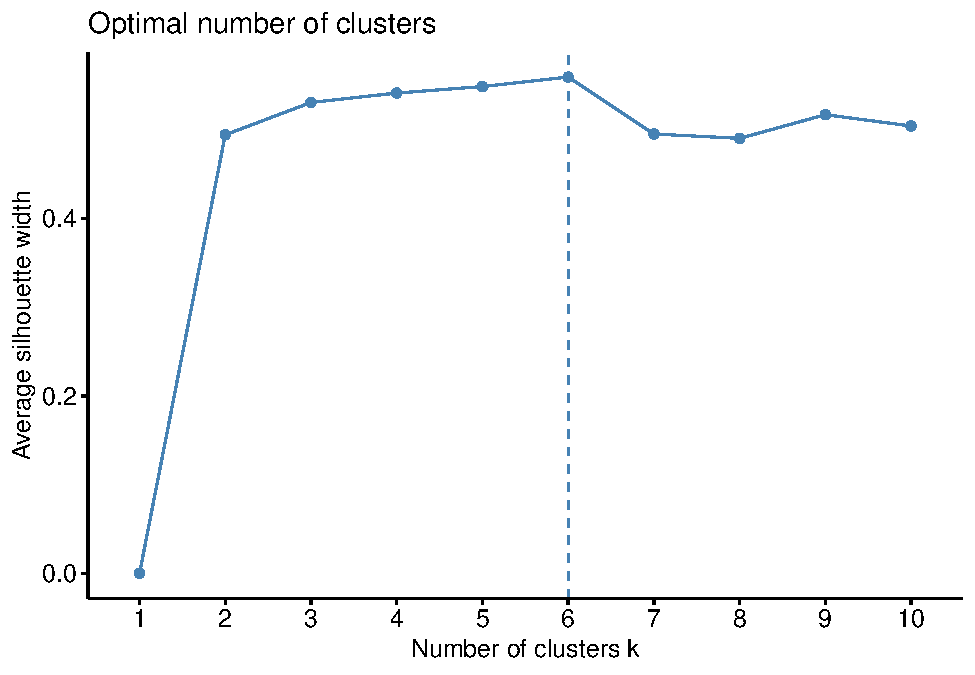
\includegraphics{Raport_finalny_files/figure-latex/unnamed-chunk-3-1.pdf}

\begin{Shaded}
\begin{Highlighting}[]
\KeywordTok{fviz_nbclust}\NormalTok{(data_train_x, kmeans, }\DataTypeTok{method =} \StringTok{"wss"}\NormalTok{)}
\end{Highlighting}
\end{Shaded}

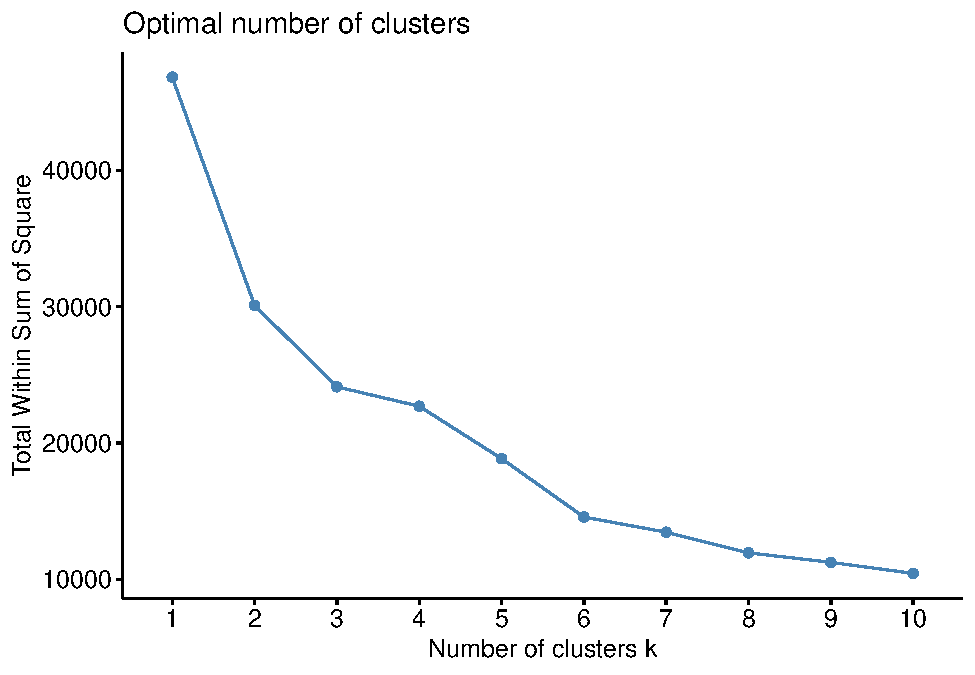
\includegraphics{Raport_finalny_files/figure-latex/unnamed-chunk-4-1.pdf}

\begin{Shaded}
\begin{Highlighting}[]
\KeywordTok{fviz_nbclust}\NormalTok{(data_train_x, kmeans, }\DataTypeTok{method =} \StringTok{"gap_stat"}\NormalTok{, }\DataTypeTok{k.max=}\DecValTok{7}\NormalTok{, }\DataTypeTok{nboot=}\DecValTok{30}\NormalTok{)}
\end{Highlighting}
\end{Shaded}

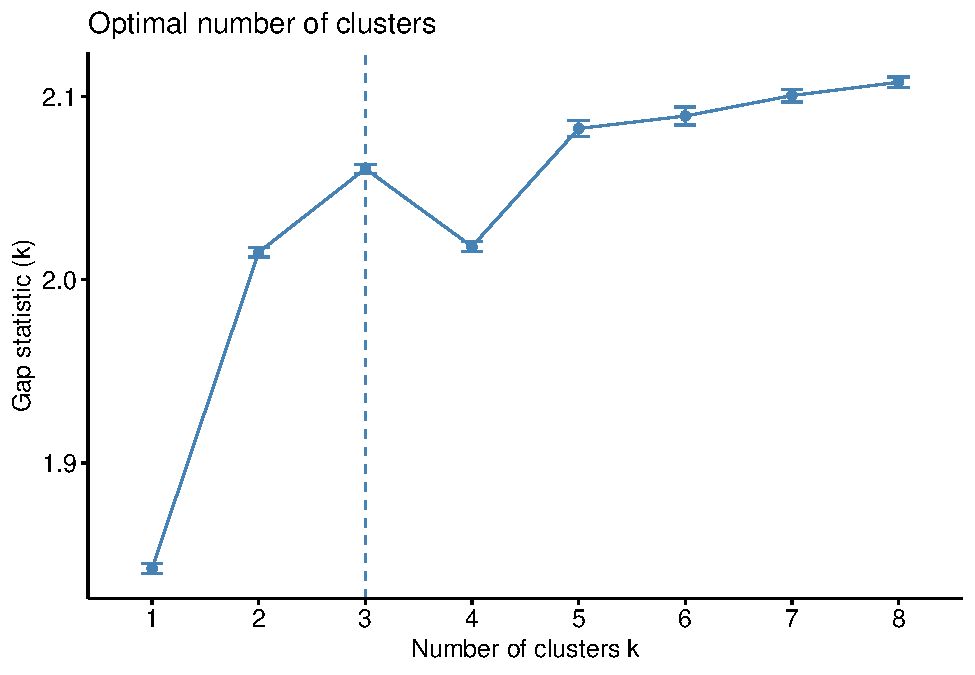
\includegraphics{Raport_finalny_files/figure-latex/number of clusters-1.pdf}

Zwizualizujmy, jak wygląda grupowanie dla wybranej ilości centroidów.

\begin{Shaded}
\begin{Highlighting}[]
\NormalTok{no_clusters =}\StringTok{ }\DecValTok{3}
\NormalTok{cluster_data =}\StringTok{ }\KeywordTok{kmeans}\NormalTok{(data_train_x, no_clusters, }\DataTypeTok{algorithm=}\StringTok{"Hartigan-Wong"}\NormalTok{)}
\KeywordTok{fviz_cluster}\NormalTok{(cluster_data, }\DataTypeTok{data =}\NormalTok{ data_train_x)}
\end{Highlighting}
\end{Shaded}

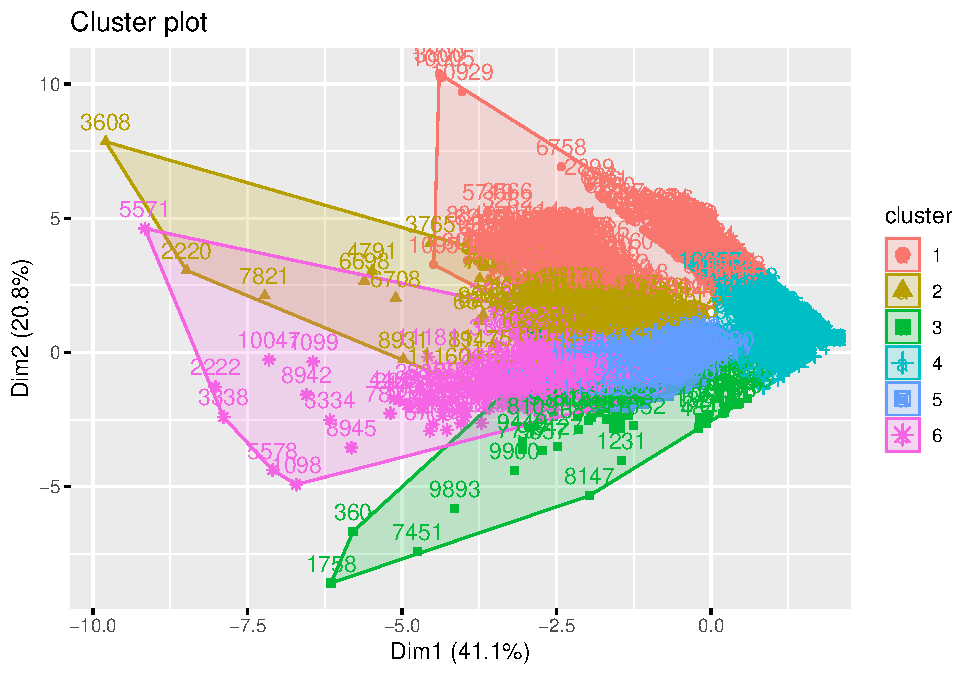
\includegraphics{Raport_finalny_files/figure-latex/unnamed-chunk-5-1.pdf}

Tutaj, aby wybrać anomalie spośród punktów w grupach należałoby dobrać
jakąś miarę niepodobieństwa. Określmy przykładową miarę niepodobieństwa
jako odległość danej od środka grupy do której została zakwalifikowana.

\begin{Shaded}
\begin{Highlighting}[]
\NormalTok{cluster_centers =}\StringTok{ }\NormalTok{cluster_data}\OperatorTok{$}\NormalTok{centers}
\NormalTok{data =}\StringTok{ }\NormalTok{data_train}
\NormalTok{data }\OperatorTok\StringTok{ }\KeywordTok{mutate}\NormalTok{(}\DataTypeTok{group =}\NormalTok{ cluster_data}\OperatorTok{$}\NormalTok{cluster) }\OperatorTok\StringTok{ }\KeywordTok{mutate}\NormalTok{(}\DataTypeTok{dist =} \KeywordTok{sqrt}\NormalTok{((V1}\OperatorTok{-}\NormalTok{cluster_centers[group, }\DecValTok{1}\NormalTok{])}\OperatorTok{^}\DecValTok{2} \OperatorTok{+}\StringTok{ }\NormalTok{(V2}\OperatorTok{-}\NormalTok{cluster_centers[group, }\DecValTok{2}\NormalTok{])}\OperatorTok{^}\DecValTok{2} \OperatorTok{+}\StringTok{ }\NormalTok{(V3}\OperatorTok{-}\NormalTok{cluster_centers[group, }\DecValTok{3}\NormalTok{])}\OperatorTok{^}\DecValTok{2} \OperatorTok{+}\StringTok{ }\NormalTok{(V4}\OperatorTok{-}\NormalTok{cluster_centers[group, }\DecValTok{4}\NormalTok{])}\OperatorTok{^}\DecValTok{2}\NormalTok{)) }\OperatorTok\StringTok{ }\KeywordTok{arrange}\NormalTok{(dist)}
\NormalTok{data}\OperatorTok{$}\NormalTok{dist =}\StringTok{ }\NormalTok{data}\OperatorTok{$}\NormalTok{dist }\OperatorTok{/}\StringTok{ }\KeywordTok{max}\NormalTok{(data}\OperatorTok{$}\NormalTok{dist)}
\KeywordTok{plot}\NormalTok{(data}\OperatorTok{$}\NormalTok{dist)}
\end{Highlighting}
\end{Shaded}

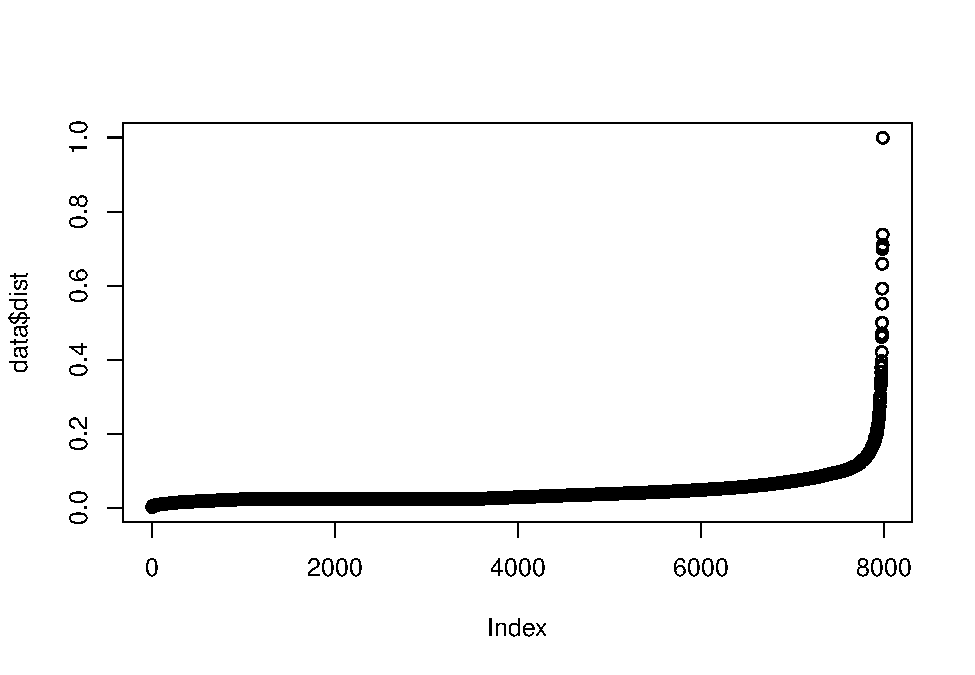
\includegraphics{Raport_finalny_files/figure-latex/unnamed-chunk-6-1.pdf}

Miara niepodobieństwa mapuje nam dane wielowymiarowe na jeden wymiar.
Zwracają one liczby w zakresie {[}0, +inf). Ustalenie wartości odcięcia
na takim zakresie jest niewygodne, postanowiliśmy ją więc znormalizować.
Użyliśmy normalizacji metodą min-max, jako że minimum tak czy inaczej
mieliśmy w zerze, to po prostu dzielimy wyniki przez ich maksimum.

\begin{Shaded}
\begin{Highlighting}[]
\KeywordTok{plot_ly}\NormalTok{(data,}
        \DataTypeTok{x =} \OperatorTok{~}\NormalTok{V1,}
        \DataTypeTok{y =} \OperatorTok{~}\NormalTok{V2,}
        \DataTypeTok{color=}\OperatorTok{~}\NormalTok{dist,}
        \DataTypeTok{colors=}\KeywordTok{c}\NormalTok{(}\StringTok{'#ffff00'}\NormalTok{, }\StringTok{'#000000'}\NormalTok{),}
        \DataTypeTok{opacity=}\FloatTok{0.7}\NormalTok{,}
        \DataTypeTok{size=}\DecValTok{1}\NormalTok{,}
        \DataTypeTok{type=}\StringTok{"scatter"}\NormalTok{,}
        \DataTypeTok{mode=}\StringTok{"markers"}
\NormalTok{      )}
\end{Highlighting}
\end{Shaded}

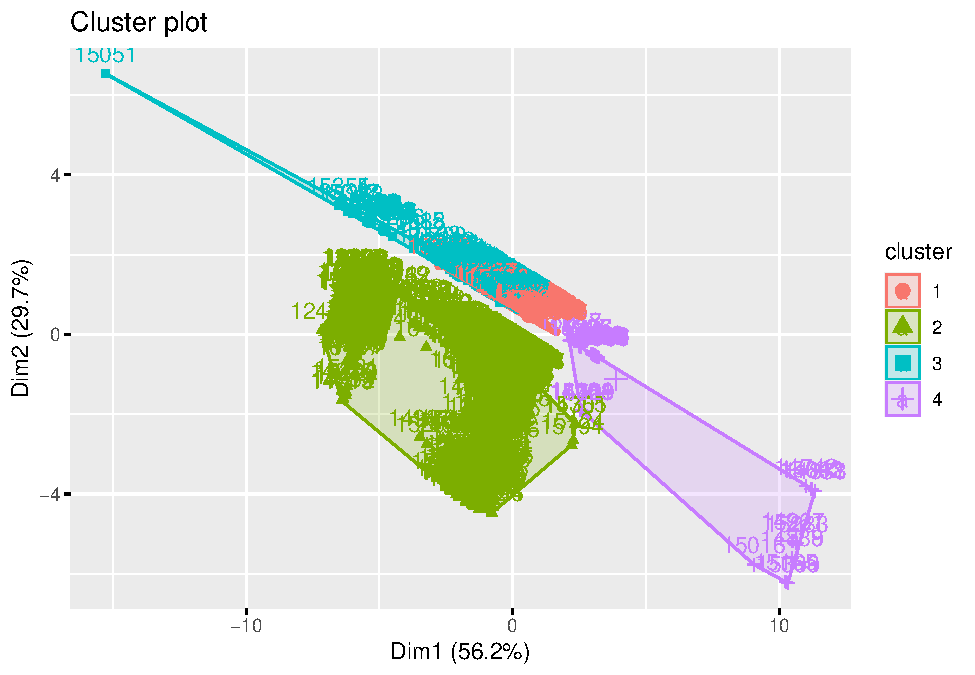
\includegraphics{Raport_finalny_files/figure-latex/unnamed-chunk-7-1.pdf}

Jednowymiarowe dane jesteśmy w stanie porównać, dzięki czemu możemy
określić jakiś próg, powyżej którego będziemy dane traktowali jako
anomalie. Po zakwalifikowaniu anomalii, możemy porównać wyniki z
faktycznie wykrytymi anomaliami podanymi w danych wejściowych. W ten
sposób dowiemy się, jaka jest jakość modelu a-priori. Na tym etapie
wybieramy jakimi miarami jakości chcielibyśmy się posłużyć. W naszym
przypadku wybieramy analizę ROC oraz miarę F1.

\begin{Shaded}
\begin{Highlighting}[]
\NormalTok{outlier_threshold =}\StringTok{ }\FloatTok{0.35}
\NormalTok{data =}\StringTok{ }\NormalTok{data }\OperatorTok\StringTok{ }\KeywordTok{mutate}\NormalTok{(}\DataTypeTok{pred_int =} \KeywordTok{as.integer}\NormalTok{(dist }\OperatorTok{>}\StringTok{ }\NormalTok{outlier_threshold))}

\NormalTok{pred =}\StringTok{ }\KeywordTok{prediction}\NormalTok{(}\DataTypeTok{predictions=}\NormalTok{data}\OperatorTok{$}\NormalTok{dist, }\DataTypeTok{labels=}\NormalTok{data}\OperatorTok{$}\NormalTok{class)}
\NormalTok{perf =}\StringTok{ }\KeywordTok{performance}\NormalTok{(pred, }\StringTok{"tpr"}\NormalTok{, }\StringTok{"fpr"}\NormalTok{)}
\KeywordTok{plot}\NormalTok{(perf)}
\KeywordTok{abline}\NormalTok{(}\DecValTok{0}\NormalTok{,}\DecValTok{1}\NormalTok{,}\DataTypeTok{col=}\StringTok{"#0000ff"}\NormalTok{)}
\end{Highlighting}
\end{Shaded}

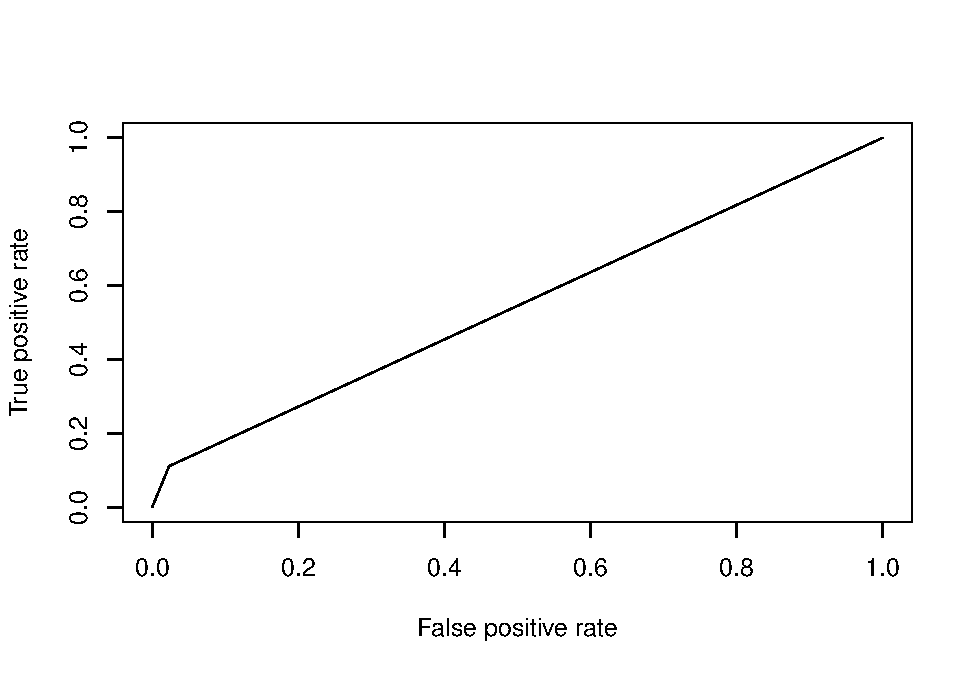
\includegraphics{Raport_finalny_files/figure-latex/unnamed-chunk-8-1.pdf}

Sprawdźmy jeszcze miarę F1. Zwraca wysokie wyniki tylko, gdy jednoczenie
oba współczynniki, precyzji i odzysku, dają wysokie wyniki.

\begin{Shaded}
\begin{Highlighting}[]
\NormalTok{data =}\StringTok{ }\NormalTok{data }\OperatorTok\StringTok{ }\KeywordTok{mutate}\NormalTok{(}\DataTypeTok{tp =}\NormalTok{ class }\OperatorTok{&}\StringTok{ }\NormalTok{pred_int)}
\NormalTok{data =}\StringTok{ }\NormalTok{data }\OperatorTok\StringTok{ }\KeywordTok{mutate}\NormalTok{(}\DataTypeTok{fp =} \OperatorTok{!}\NormalTok{class }\OperatorTok{&}\StringTok{ }\NormalTok{pred_int)}
\NormalTok{data =}\StringTok{ }\NormalTok{data }\OperatorTok\StringTok{ }\KeywordTok{mutate}\NormalTok{(}\DataTypeTok{tn =} \OperatorTok{!}\NormalTok{class }\OperatorTok{&}\StringTok{ }\OperatorTok{!}\NormalTok{pred_int)}
\NormalTok{data =}\StringTok{ }\NormalTok{data }\OperatorTok\StringTok{ }\KeywordTok{mutate}\NormalTok{(}\DataTypeTok{fn =}\NormalTok{ class }\OperatorTok{&}\StringTok{ }\OperatorTok{!}\NormalTok{pred_int)}
\NormalTok{recall =}\StringTok{ }\KeywordTok{tally}\NormalTok{(data, tp) }\OperatorTok{/}\StringTok{ }\NormalTok{(}\KeywordTok{tally}\NormalTok{(data, tp) }\OperatorTok{+}\StringTok{ }\KeywordTok{tally}\NormalTok{(data, fn))}
\NormalTok{precision =}\StringTok{ }\KeywordTok{tally}\NormalTok{(data, tp) }\OperatorTok{/}\StringTok{ }\NormalTok{(}\KeywordTok{tally}\NormalTok{(data, tp) }\OperatorTok{+}\StringTok{ }\KeywordTok{tally}\NormalTok{(data, fp))}
\NormalTok{f_value =}\StringTok{ }\DecValTok{2} \OperatorTok{*}\StringTok{ }\NormalTok{recall }\OperatorTok{*}\StringTok{ }\NormalTok{precision }\OperatorTok{/}\StringTok{ }\NormalTok{(recall }\OperatorTok{+}\StringTok{ }\NormalTok{precision)}
\NormalTok{f_value}
\end{Highlighting}
\end{Shaded}

\begin{verbatim}
##            n
## 1 0.01010101
\end{verbatim}

Na tym etapie mamy wyniki jakie metody grupowania mogłyby dać dla tego
zbioru danych. Są to niestety miary które niewiele mówią o jakości
predykcji dla nowych danych. Są one w zasadzie tylko poglądowe, aby
upewnić się że można wytrenować model w sposób nienadzorowany metodami
grupowania, tak aby wyniki detekcji anomalii na podstawie tego modelu
były nielosowe i relatywnie poprawne.

W tym miejscu warto zaznaczyć, że wynik NaN oznacza, że i precyzja i
odzysk osiągnęły wartość 0, czyli nie było poprawnie zakwalifikowanej
nawet jednej anomalii. W pozostałych przypadkach, określona wartość
będzie plasowała się w przedziale {[}0,1{]}, gdzie 0 będzie oznaczało
jakość niską, a 1 wysoką.

Natomiast, aby określić jakość modelu, musielibyśmy zastosować go dla
nowych danych i sprawdzić czy predykcje okazałyby się identyczne z
faktycznym wynikiem kwalifikacji anomalii.

Aby określić jak model radzi sobie z nowymi danymi, będziemy musieli go
zastosować dla zbioru danych który nie został wzięty pod uwagę przy
tworzeniu modelu.

\begin{Shaded}
\begin{Highlighting}[]
\NormalTok{outlier_threshold =}\StringTok{ }\FloatTok{0.4}
\NormalTok{predict.kmeans <-}\StringTok{ }\ControlFlowTok{function}\NormalTok{(object, newdata)\{}
\NormalTok{    centers <-}\StringTok{ }\NormalTok{object}\OperatorTok{$}\NormalTok{centers}
\NormalTok{    n_centers <-}\StringTok{ }\KeywordTok{nrow}\NormalTok{(centers)}
\NormalTok{    dist_mat <-}\StringTok{ }\KeywordTok{as.matrix}\NormalTok{(}\KeywordTok{dist}\NormalTok{(}\KeywordTok{rbind}\NormalTok{(centers, newdata)))}
\NormalTok{    dist_mat <-}\StringTok{ }\NormalTok{dist_mat[}\OperatorTok{-}\KeywordTok{seq}\NormalTok{(n_centers), }\KeywordTok{seq}\NormalTok{(n_centers)]}
    \KeywordTok{max.col}\NormalTok{(}\OperatorTok{-}\NormalTok{dist_mat)}
\NormalTok{\}}

\NormalTok{groups =}\StringTok{ }\KeywordTok{predict}\NormalTok{(cluster_data, data_test_x)}
\NormalTok{data =}\StringTok{ }\NormalTok{data_test }\OperatorTok\StringTok{ }\KeywordTok{mutate}\NormalTok{(}\DataTypeTok{group =}\NormalTok{ groups)}
\NormalTok{data }\OperatorTok\StringTok{ }\KeywordTok{mutate}\NormalTok{(}\DataTypeTok{dist =} \KeywordTok{sqrt}\NormalTok{((V1}\OperatorTok{-}\NormalTok{cluster_centers[group, }\DecValTok{1}\NormalTok{])}\OperatorTok{^}\DecValTok{2} \OperatorTok{+}\StringTok{ }\NormalTok{(V2}\OperatorTok{-}\NormalTok{cluster_centers[group, }\DecValTok{2}\NormalTok{])}\OperatorTok{^}\DecValTok{2} \OperatorTok{+}\StringTok{ }\NormalTok{(V3}\OperatorTok{-}\NormalTok{cluster_centers[group, }\DecValTok{3}\NormalTok{])}\OperatorTok{^}\DecValTok{2} \OperatorTok{+}\StringTok{ }\NormalTok{(V4}\OperatorTok{-}\NormalTok{cluster_centers[group, }\DecValTok{4}\NormalTok{])}\OperatorTok{^}\DecValTok{2}\NormalTok{)) }\OperatorTok\StringTok{ }\KeywordTok{arrange}\NormalTok{(dist)}
\NormalTok{data}\OperatorTok{$}\NormalTok{dist =}\StringTok{ }\NormalTok{data}\OperatorTok{$}\NormalTok{dist }\OperatorTok{/}\StringTok{ }\KeywordTok{max}\NormalTok{(data}\OperatorTok{$}\NormalTok{dist)}
\NormalTok{data =}\StringTok{ }\NormalTok{data }\OperatorTok\StringTok{ }\KeywordTok{mutate}\NormalTok{(}\DataTypeTok{pred_int =} \KeywordTok{as.integer}\NormalTok{(dist }\OperatorTok{>}\StringTok{ }\NormalTok{outlier_threshold))}
\KeywordTok{plot}\NormalTok{(data}\OperatorTok{$}\NormalTok{dist)}
\end{Highlighting}
\end{Shaded}

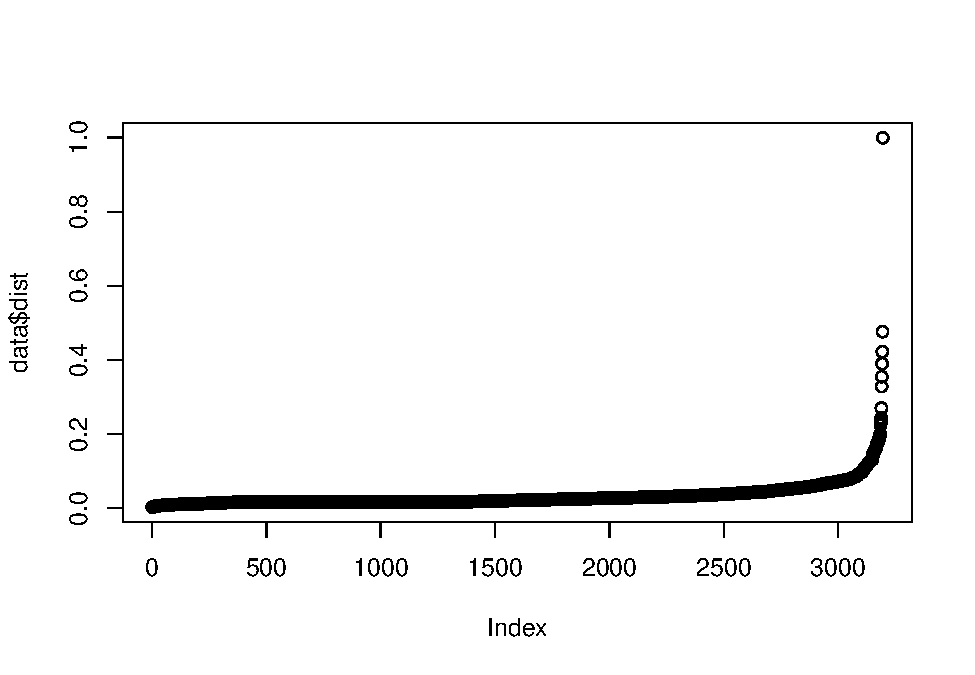
\includegraphics{Raport_finalny_files/figure-latex/unnamed-chunk-10-1.pdf}

Zrobiliśmy predykcje grup na podstawie modelu, zaaplikowaliśmy miarę
niepodobieństwa na wyniki danych testowych. Rozkład posortowanych miar
niepodobieństwa dla danych testowych prezentuje się jak wyżej.

Aby określić jakość predykcji, zastosujemy analizę roc oraz wyliczymy
miarę F1.

\begin{Shaded}
\begin{Highlighting}[]
\NormalTok{pred =}\StringTok{ }\KeywordTok{prediction}\NormalTok{(}\DataTypeTok{predictions=}\NormalTok{data}\OperatorTok{$}\NormalTok{dist, }\DataTypeTok{labels=}\NormalTok{data}\OperatorTok{$}\NormalTok{class)}
\NormalTok{perf =}\StringTok{ }\KeywordTok{performance}\NormalTok{(pred, }\StringTok{"tpr"}\NormalTok{, }\StringTok{"fpr"}\NormalTok{)}
\KeywordTok{plot}\NormalTok{(perf)}
\KeywordTok{abline}\NormalTok{(}\DecValTok{0}\NormalTok{,}\DecValTok{1}\NormalTok{,}\DataTypeTok{col=}\StringTok{"#0000ff"}\NormalTok{)}
\end{Highlighting}
\end{Shaded}

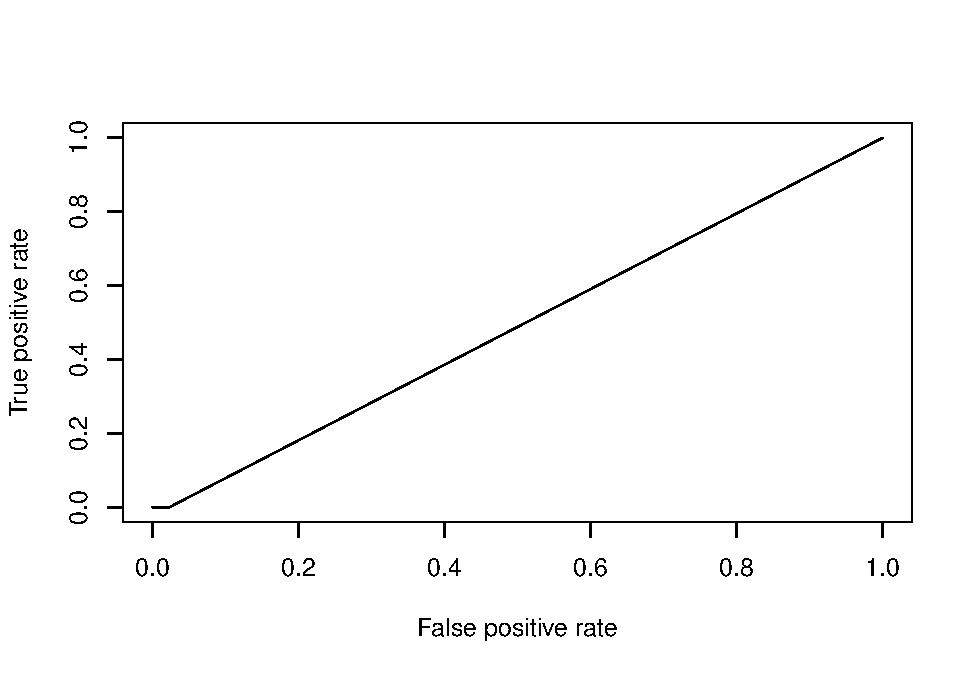
\includegraphics{Raport_finalny_files/figure-latex/unnamed-chunk-11-1.pdf}

\begin{Shaded}
\begin{Highlighting}[]
\NormalTok{data =}\StringTok{ }\NormalTok{data }\OperatorTok\StringTok{ }\KeywordTok{mutate}\NormalTok{(}\DataTypeTok{tp =}\NormalTok{ class }\OperatorTok{&}\StringTok{ }\NormalTok{pred_int)}
\NormalTok{data =}\StringTok{ }\NormalTok{data }\OperatorTok\StringTok{ }\KeywordTok{mutate}\NormalTok{(}\DataTypeTok{fp =} \OperatorTok{!}\NormalTok{class }\OperatorTok{&}\StringTok{ }\NormalTok{pred_int)}
\NormalTok{data =}\StringTok{ }\NormalTok{data }\OperatorTok\StringTok{ }\KeywordTok{mutate}\NormalTok{(}\DataTypeTok{tn =} \OperatorTok{!}\NormalTok{class }\OperatorTok{&}\StringTok{ }\OperatorTok{!}\NormalTok{pred_int)}
\NormalTok{data =}\StringTok{ }\NormalTok{data }\OperatorTok\StringTok{ }\KeywordTok{mutate}\NormalTok{(}\DataTypeTok{fn =}\NormalTok{ class }\OperatorTok{&}\StringTok{ }\OperatorTok{!}\NormalTok{pred_int)}
\NormalTok{recall =}\StringTok{ }\KeywordTok{tally}\NormalTok{(data, tp) }\OperatorTok{/}\StringTok{ }\NormalTok{(}\KeywordTok{tally}\NormalTok{(data, tp) }\OperatorTok{+}\StringTok{ }\KeywordTok{tally}\NormalTok{(data, fn))}
\NormalTok{precision =}\StringTok{ }\KeywordTok{tally}\NormalTok{(data, tp) }\OperatorTok{/}\StringTok{ }\NormalTok{(}\KeywordTok{tally}\NormalTok{(data, tp) }\OperatorTok{+}\StringTok{ }\KeywordTok{tally}\NormalTok{(data, fp))}
\NormalTok{f_value =}\StringTok{ }\DecValTok{2} \OperatorTok{*}\StringTok{ }\NormalTok{recall }\OperatorTok{*}\StringTok{ }\NormalTok{precision }\OperatorTok{/}\StringTok{ }\NormalTok{(recall }\OperatorTok{+}\StringTok{ }\NormalTok{precision)}
\NormalTok{f_value}
\end{Highlighting}
\end{Shaded}

\begin{verbatim}
##     n
## 1 NaN
\end{verbatim}

Miary jakości powyżej oznaczają, że detekcja anomalii z użyciem takich
parametrów, miary niepodobieństwa w postaci odległości od najbliższego
klastra i z zastosowaniem grupowania centroidami nie przynosi znaczącego
uzysku ponad losowe wybieranie anomalii spośród danych. Może być to
spowodowane, że algorytm centroidów jest słabo dostosowany do
charakterystyki danych tego zbioru, jak również słabym dopasowaniem
miary niepodobieństwa.

Możliwe, że w przypadku tego zbioru danych zastosowanie innych
algorytmów grupowania oraz innych miar niepodobieństwa do grup okazałoby
się jakościowo lepszym rozwiązaniem.

\hypertarget{klasyfikacja}{%
\subsubsection{Klasyfikacja}\label{klasyfikacja}}

Na tych samych zbiorach danych uruchomiono nadzorowane algorytmy
klasyfikacji w celu porównania ich skuteczności z algorytmami
grupującymi uczonymi bez nadzoru. W tym celu wykorzystano wbudowane
metody klasyfikacji: * \texttt{svm} (Support Vector Machine) z funkcją
jądrową wielomianową * \texttt{naiveBayes} (Naiwny klasyfikator
Bayesowski) * \texttt{ctree} (Conditional Inference Tree)

Do każdej z metod podano wartości ze zbioru treningowego wraz z etykietą
przynależności do klasy anomalii, a następnie dokonano predyckji klasy
dla punktów ze zbioru testowego. Zbiory były takie same jak podczas
nienadzorowanego grupowania.

Dla każdej z metod dokonano pomiaru wskażnika F na podstawie macierzy
błędów oraz wyznaczono kształt krzywej ROC.

Do określania miary F1 użyliśmy definicji funkcji:

\begin{Shaded}
\begin{Highlighting}[]
\NormalTok{f_value <-}\StringTok{ }\ControlFlowTok{function}\NormalTok{ (cm) \{}
\NormalTok{  fp =}\StringTok{ }\NormalTok{cm[}\DecValTok{1}\NormalTok{,}\DecValTok{2}\NormalTok{]}
\NormalTok{  fn =}\StringTok{ }\NormalTok{cm[}\DecValTok{2}\NormalTok{,}\DecValTok{1}\NormalTok{]}
\NormalTok{  tp =}\StringTok{ }\NormalTok{cm[}\DecValTok{2}\NormalTok{,}\DecValTok{2}\NormalTok{]}
\NormalTok{  recall =}\StringTok{ }\NormalTok{tp }\OperatorTok{/}\StringTok{ }\NormalTok{(tp}\OperatorTok{+}\NormalTok{fn)}
\NormalTok{  precision =}\StringTok{ }\NormalTok{tp }\OperatorTok{/}\StringTok{ }\NormalTok{(tp}\OperatorTok{+}\NormalTok{fp)}
\NormalTok{  f =}\StringTok{ }\NormalTok{(}\DecValTok{2} \OperatorTok{*}\StringTok{ }\NormalTok{recall }\OperatorTok{*}\StringTok{ }\NormalTok{precision) }\OperatorTok{/}\StringTok{ }\NormalTok{(recall }\OperatorTok{+}\StringTok{ }\NormalTok{precision)}
  \KeywordTok{return}\NormalTok{(f)}
\NormalTok{\}}
\end{Highlighting}
\end{Shaded}

\hypertarget{algorytmy}{%
\paragraph{Algorytmy}\label{algorytmy}}

\hypertarget{support-vector-machines-svm}{%
\subparagraph{Support Vector Machines
(SVM)}\label{support-vector-machines-svm}}

Metoda ma za zadanie wyznaczyć hiperpłaszczyznę oddzielającą przykłady
należące do dwóch klas w taki sposób aby uzyskać między nimi największy
margines. Funkcja jądrowa ma zadanie przekształcić dane wejściowe do
takiej przestrzeni, aby możliwe było wyznaczenie płaszczyzny która
oddziela najwięcej punktów.

\begin{Shaded}
\begin{Highlighting}[]
\NormalTok{svm.model =}\StringTok{ }\KeywordTok{svm}\NormalTok{(}\KeywordTok{as.factor}\NormalTok{(class) }\OperatorTok{~}\StringTok{ }\NormalTok{., }\DataTypeTok{data =}\NormalTok{ data_train, }\DataTypeTok{type =} \StringTok{'C-classification'}\NormalTok{, }\DataTypeTok{kernel =} \StringTok{'polynomial'}\NormalTok{, }\DataTypeTok{probability =} \OtherTok{TRUE}\NormalTok{)}
\NormalTok{svm.pred =}\StringTok{ }\KeywordTok{predict}\NormalTok{(svm.model, }\DataTypeTok{newdata =}\NormalTok{ data_test_x)}
\NormalTok{svm.cm =}\StringTok{ }\KeywordTok{table}\NormalTok{(data_test_y}\OperatorTok{$}\NormalTok{class, svm.pred)}
\KeywordTok{f_value}\NormalTok{(svm.cm)}
\end{Highlighting}
\end{Shaded}

\begin{verbatim}
## [1] 0.6086957
\end{verbatim}

\hypertarget{naiwny-klasyfikator-bayesowski}{%
\subparagraph{Naiwny klasyfikator
Bayesowski}\label{naiwny-klasyfikator-bayesowski}}

Metoda zakłada niezależność zmiennych decyzyjnych, i wyznacza na ich
podstawie prawdopodobieństwo przynależności przynależności punktu
wejściowego do danej klasy, tworząc modele rozkładów ze na podstawie
przykładów ze zbioru uczącego. Ponieważ jedną z dwu klas stanowią
anomalie, modelowanie ich rozkładu z definiji powinno okazać się
nieskuteczne.

\begin{Shaded}
\begin{Highlighting}[]
\NormalTok{nvb.model =}\StringTok{ }\KeywordTok{naiveBayes}\NormalTok{(}\KeywordTok{as.factor}\NormalTok{(class) }\OperatorTok{~}\StringTok{ }\NormalTok{., }\DataTypeTok{data =}\NormalTok{ data_train)}
\NormalTok{nvb.pred =}\StringTok{ }\KeywordTok{predict}\NormalTok{(nvb.model, }\DataTypeTok{newdata =}\NormalTok{ data_test_x)}
\NormalTok{nvb.cm =}\StringTok{ }\KeywordTok{table}\NormalTok{(data_test_y}\OperatorTok{$}\NormalTok{class, nvb.pred)}
\KeywordTok{f_value}\NormalTok{(nvb.cm)}
\end{Highlighting}
\end{Shaded}

\begin{verbatim}
## [1] 0.3700787
\end{verbatim}

\hypertarget{conditional-inference-tree-ctree}{%
\subparagraph{Conditional Inference Tree
(ctree)}\label{conditional-inference-tree-ctree}}

Drzewo wnioskowania warunkowego jest drzewem decyzyjnym konstruującym
kolejne poziomy podziału na podstawie statystycznego testu niezależności
zmiennych decyzyjnych od klasy. Dla każdego poziomu decyzji wybierana
jest ta zmienna decyzyjna dla której test niezależności klasy od
zmiennej ma najwyższą istotność (zmienna jest silnie związana z klasą).
Tak skonstuowane drzewo nie wymaga dlaszego przycinania.

\begin{Shaded}
\begin{Highlighting}[]
\NormalTok{ct.model =}\StringTok{ }\KeywordTok{ctree}\NormalTok{(}\KeywordTok{as.factor}\NormalTok{(class) }\OperatorTok{~}\StringTok{ }\NormalTok{., }\DataTypeTok{data =}\NormalTok{ data_train)}
\NormalTok{ct.pred =}\StringTok{ }\KeywordTok{predict}\NormalTok{(ct.model, }\DataTypeTok{newdata =}\NormalTok{ data_test_x)}
\NormalTok{ct.cm =}\StringTok{ }\KeywordTok{table}\NormalTok{(data_test_y}\OperatorTok{$}\NormalTok{class, ct.pred)}
\KeywordTok{f_value}\NormalTok{(ct.cm)}
\end{Highlighting}
\end{Shaded}

\begin{verbatim}
## [1] 0.5511811
\end{verbatim}

\hypertarget{jakoux15bux107-modeli}{%
\paragraph{Jakość modeli}\label{jakoux15bux107-modeli}}

Analiza ROC pozwala nam zobaczyć jakość predykcji danego algorytmu. Im
większe jest pole pod wykresem, tym wyższa jakość modelu.

\begin{Shaded}
\begin{Highlighting}[]
\KeywordTok{require}\NormalTok{(ROCR)}
\NormalTok{svm.prob =}\StringTok{ }\KeywordTok{predict}\NormalTok{(svm.model, }\DataTypeTok{type=}\StringTok{"prob"}\NormalTok{, }\DataTypeTok{newdata=}\NormalTok{ data_test_x, }\DataTypeTok{probability =} \OtherTok{TRUE}\NormalTok{)}
\NormalTok{svm.rocr =}\StringTok{ }\KeywordTok{prediction}\NormalTok{(}\KeywordTok{attr}\NormalTok{(svm.prob, }\StringTok{"probabilities"}\NormalTok{)[,}\DecValTok{2}\NormalTok{], data_test_y}\OperatorTok{$}\NormalTok{class)}
\NormalTok{svm.perf =}\StringTok{ }\KeywordTok{performance}\NormalTok{(svm.rocr, }\StringTok{"tpr"}\NormalTok{,}\StringTok{"fpr"}\NormalTok{)}
\NormalTok{nvb.prob =}\StringTok{ }\KeywordTok{predict}\NormalTok{(nvb.model, }\DataTypeTok{newdata=}\NormalTok{data_test_x, }\DataTypeTok{type=}\StringTok{"raw"}\NormalTok{)}
\NormalTok{nvb.rocr =}\StringTok{ }\KeywordTok{prediction}\NormalTok{(nvb.prob[,}\DecValTok{2}\NormalTok{], data_test_y}\OperatorTok{$}\NormalTok{class)}
\NormalTok{nvb.perf =}\StringTok{ }\KeywordTok{performance}\NormalTok{(nvb.rocr, }\StringTok{"tpr"}\NormalTok{,}\StringTok{"fpr"}\NormalTok{)}
\NormalTok{ct.prob =}\StringTok{ }\KeywordTok{predict}\NormalTok{(ct.model, }\DataTypeTok{newdata=}\NormalTok{data_test_x, }\DataTypeTok{type=}\StringTok{"prob"}\NormalTok{)}
\NormalTok{ct.rocr =}\StringTok{ }\KeywordTok{prediction}\NormalTok{(ct.prob[,}\DecValTok{2}\NormalTok{], data_test_y}\OperatorTok{$}\NormalTok{class)}
\NormalTok{ct.perf =}\StringTok{ }\KeywordTok{performance}\NormalTok{(ct.rocr, }\StringTok{"tpr"}\NormalTok{,}\StringTok{"fpr"}\NormalTok{)}
\KeywordTok{plot}\NormalTok{(svm.perf, }\DataTypeTok{col=}\DecValTok{4}\NormalTok{, }\DataTypeTok{main=}\StringTok{"ROC curves of different machine learning classifier"}\NormalTok{)}
\KeywordTok{legend}\NormalTok{(}\FloatTok{0.6}\NormalTok{, }\FloatTok{0.6}\NormalTok{, }\KeywordTok{c}\NormalTok{(}\StringTok{'svm'}\NormalTok{, }\StringTok{'ctree'}\NormalTok{, }\StringTok{'Naive Bayes'}\NormalTok{), }\DecValTok{4}\OperatorTok{:}\DecValTok{6}\NormalTok{)}
\KeywordTok{plot}\NormalTok{(ct.perf, }\DataTypeTok{col=}\DecValTok{5}\NormalTok{, }\DataTypeTok{add=}\OtherTok{TRUE}\NormalTok{)}
\KeywordTok{plot}\NormalTok{(nvb.perf, }\DataTypeTok{col=}\DecValTok{6}\NormalTok{, }\DataTypeTok{add=}\OtherTok{TRUE}\NormalTok{)}
\end{Highlighting}
\end{Shaded}

\includegraphics{Raport_finalny_files/figure-latex/unnamed-chunk-17-1.pdf}

\hypertarget{przebieg-badania}{%
\subsection{Przebieg badania}\label{przebieg-badania}}

\hypertarget{poruxf3wnanie-algorytmuxf3w-grupowania-cmeans-kmeans-dla-miar-niepodobieux144stwa-cblof-ucblof-i-ldcof-wzglux119dem-klasyfikacji-algorytmami-svm-naive-bayes-i-ctree}{%
\subsubsection{Porównanie algorytmów grupowania cmeans, kmeans dla miar
niepodobieństwa CBLOF, uCBLOF i LDCOF względem klasyfikacji algorytmami
SVM, Naive-Bayes i
CTree}\label{poruxf3wnanie-algorytmuxf3w-grupowania-cmeans-kmeans-dla-miar-niepodobieux144stwa-cblof-ucblof-i-ldcof-wzglux119dem-klasyfikacji-algorytmami-svm-naive-bayes-i-ctree}}

\hypertarget{zaux142oux17cenia}{%
\paragraph{Założenia}\label{zaux142oux17cenia}}

W tym dokumencie chcemy się skupić na porównaniu doboru miary
niepodobieństwa i algorytmu grupowania, a wynikami wybranych algorytmów
klasyfikacji. W związku z tym, porównania będziemy wykonywać już na
dobranych parametrach. Nie zapewniamy, że parametry zostały dobrane
idealnie do podanych zbiorów danych i z użyciem odpowiednich narzędzi.
Dobór parametrów został wykonany dla każdego zbioru danych oddzielnie.
Sposób doboru parametrów został opisany w oddzielnym pliku.

\hypertarget{przebieg-badania-1}{%
\paragraph{Przebieg badania}\label{przebieg-badania-1}}

Zaczytamy najpierw dane dwóch zbiorów danych, oba mają dane 6-wymiarowe.
Zbiór mammography składa się z 11183 rekordów, z czego 260 to anomalie.
Zbiór annthyroid składa się z 7200 rekordów, z czego 534 to anomalie

\begin{Shaded}
\begin{Highlighting}[]
\KeywordTok{rm}\NormalTok{(}\DataTypeTok{list =} \KeywordTok{ls}\NormalTok{())}
\NormalTok{mammography_x =}\StringTok{ }\KeywordTok{read.csv}\NormalTok{(}\DataTypeTok{file =} \StringTok{'mammography_x.csv'}\NormalTok{, }\DataTypeTok{header=}\OtherTok{FALSE}\NormalTok{)}
\NormalTok{mammography_y =}\StringTok{ }\KeywordTok{read.csv}\NormalTok{(}\DataTypeTok{file =} \StringTok{'mammography_y.csv'}\NormalTok{, }\DataTypeTok{header=}\OtherTok{FALSE}\NormalTok{)}
\NormalTok{mammography =}\StringTok{ }\NormalTok{mammography_x }\OperatorTok\StringTok{ }\KeywordTok{mutate}\NormalTok{(}\DataTypeTok{class =}\NormalTok{ mammography_y}\OperatorTok{$}\NormalTok{V1)}

\NormalTok{annthyroid_x =}\StringTok{ }\KeywordTok{read.csv}\NormalTok{(}\DataTypeTok{file =} \StringTok{'annthyroid_x.csv'}\NormalTok{, }\DataTypeTok{header=}\OtherTok{FALSE}\NormalTok{)}
\NormalTok{annthyroid_y =}\StringTok{ }\KeywordTok{read.csv}\NormalTok{(}\DataTypeTok{file =} \StringTok{'annthyroid_y.csv'}\NormalTok{, }\DataTypeTok{header=}\OtherTok{FALSE}\NormalTok{)}
\NormalTok{annthyroid =}\StringTok{ }\NormalTok{annthyroid_x }\OperatorTok\StringTok{ }\KeywordTok{mutate}\NormalTok{(}\DataTypeTok{class =}\NormalTok{ annthyroid_y}\OperatorTok{$}\NormalTok{V1)}
\end{Highlighting}
\end{Shaded}

Wyniki poszczególnych bloków kodu będą przedstawiały odpowiednio: -
wykres wstępnie wizualizujący efekty grupowania, - wykres
przedstawiający rozkład wyników pomiaru niepodobieństwa do dopasowanych
grup dla poszczególnych punktów ze zbioru danych, - wynik pomiaru
współczynnika F dla zadanej wartości odcięcia, - wykres ROC

Wewnątrz bloków kodu będziemy ustalać podział dla danych treningowych i
testowych, określać z którego algorytmu będziemy korzystać, podawać
hiperparametry niezbędne do jego działania oraz dodatkowo określać
poziom odcięcia miary niepodobieństwa, od którego będziemy uznawać
punkty jako anomalie.

\hypertarget{poruxf3wnanie-wpux142ywu-miary-niepodobieux144stwa}{%
\subparagraph{Porównanie wpływu miary
niepodobieństwa}\label{poruxf3wnanie-wpux142ywu-miary-niepodobieux144stwa}}

Sprawdźmy najpierw w ramach pierwszego zbioru danych, jaki wpływ na
wynik ma dobór miary niepodobieństwa.

\begin{Shaded}
\begin{Highlighting}[]
\NormalTok{split_ratio =}\StringTok{ }\FloatTok{0.8}
\KeywordTok{set.seed}\NormalTok{(}\DecValTok{123}\NormalTok{)}
\NormalTok{split =}\StringTok{ }\KeywordTok{sample.split}\NormalTok{(mammography, }\DataTypeTok{SplitRatio =}\NormalTok{ split_ratio)}
\NormalTok{data_train =}\StringTok{ }\KeywordTok{subset}\NormalTok{(mammography, split }\OperatorTok{==}\StringTok{ }\OtherTok{TRUE}\NormalTok{)}
\NormalTok{data_test =}\StringTok{ }\KeywordTok{subset}\NormalTok{(mammography, split }\OperatorTok{==}\StringTok{ }\OtherTok{FALSE}\NormalTok{)}

\NormalTok{metric =}\StringTok{ "euclidean"}
\NormalTok{method =}\StringTok{ "kmeans"}
\NormalTok{dissimilarity_measure =}\StringTok{ "uCBLOF"}
\NormalTok{no_clusters =}\StringTok{ }\DecValTok{6}
\NormalTok{algorithm =}\StringTok{ "Hartigan-Wong"}
\NormalTok{outlier_threshold =}\StringTok{ }\FloatTok{0.3}
\KeywordTok{source}\NormalTok{(}\StringTok{"Interface.R"}\NormalTok{, }\DataTypeTok{local=}\NormalTok{knitr}\OperatorTok{::}\KeywordTok{knit_global}\NormalTok{(), }\DataTypeTok{echo=}\OtherTok{FALSE}\NormalTok{)}
\end{Highlighting}
\end{Shaded}

\includegraphics{Raport_finalny_files/figure-latex/unnamed-chunk-18-1.pdf}
\includegraphics{Raport_finalny_files/figure-latex/unnamed-chunk-18-2.pdf}
\includegraphics{Raport_finalny_files/figure-latex/unnamed-chunk-18-3.pdf}

\begin{verbatim}
## [1] "F-value: 0.0246913580246914"
\end{verbatim}

\begin{Shaded}
\begin{Highlighting}[]
\NormalTok{split_ratio =}\StringTok{ }\FloatTok{0.8}
\KeywordTok{set.seed}\NormalTok{(}\DecValTok{123}\NormalTok{)}
\NormalTok{split =}\StringTok{ }\KeywordTok{sample.split}\NormalTok{(mammography, }\DataTypeTok{SplitRatio =}\NormalTok{ split_ratio)}
\NormalTok{data_train =}\StringTok{ }\KeywordTok{subset}\NormalTok{(mammography, split }\OperatorTok{==}\StringTok{ }\OtherTok{TRUE}\NormalTok{)}
\NormalTok{data_test =}\StringTok{ }\KeywordTok{subset}\NormalTok{(mammography, split }\OperatorTok{==}\StringTok{ }\OtherTok{FALSE}\NormalTok{)}

\NormalTok{metric =}\StringTok{ "euclidean"}
\NormalTok{method =}\StringTok{ "kmeans"}
\NormalTok{dissimilarity_measure =}\StringTok{ "CBLOF"}
\NormalTok{no_clusters =}\StringTok{ }\DecValTok{6}
\NormalTok{algorithm =}\StringTok{ "Hartigan-Wong"}
\NormalTok{outlier_threshold =}\StringTok{ }\FloatTok{0.3}
\KeywordTok{source}\NormalTok{(}\StringTok{"Interface.R"}\NormalTok{, }\DataTypeTok{local=}\NormalTok{knitr}\OperatorTok{::}\KeywordTok{knit_global}\NormalTok{(), }\DataTypeTok{echo=}\OtherTok{FALSE}\NormalTok{)}
\end{Highlighting}
\end{Shaded}

\begin{verbatim}
## `summarise()` ungrouping output (override with `.groups` argument)
\end{verbatim}

\includegraphics{Raport_finalny_files/figure-latex/unnamed-chunk-19-1.pdf}
\includegraphics{Raport_finalny_files/figure-latex/unnamed-chunk-19-2.pdf}
\includegraphics{Raport_finalny_files/figure-latex/unnamed-chunk-19-3.pdf}

\begin{verbatim}
## [1] "F-value: 0.0374531835205993"
\end{verbatim}

\begin{Shaded}
\begin{Highlighting}[]
\NormalTok{split_ratio =}\StringTok{ }\FloatTok{0.8}
\KeywordTok{set.seed}\NormalTok{(}\DecValTok{123}\NormalTok{)}
\NormalTok{split =}\StringTok{ }\KeywordTok{sample.split}\NormalTok{(mammography, }\DataTypeTok{SplitRatio =}\NormalTok{ split_ratio)}
\NormalTok{data_train =}\StringTok{ }\KeywordTok{subset}\NormalTok{(mammography, split }\OperatorTok{==}\StringTok{ }\OtherTok{TRUE}\NormalTok{)}
\NormalTok{data_test =}\StringTok{ }\KeywordTok{subset}\NormalTok{(mammography, split }\OperatorTok{==}\StringTok{ }\OtherTok{FALSE}\NormalTok{)}

\NormalTok{metric =}\StringTok{ "euclidean"}
\NormalTok{method =}\StringTok{ "kmeans"}
\NormalTok{dissimilarity_measure =}\StringTok{ "LDCOF"}
\NormalTok{no_clusters =}\StringTok{ }\DecValTok{6}
\NormalTok{algorithm =}\StringTok{ "Hartigan-Wong"}
\NormalTok{outlier_threshold =}\StringTok{ }\FloatTok{0.5}
\KeywordTok{source}\NormalTok{(}\StringTok{"Interface.R"}\NormalTok{, }\DataTypeTok{local=}\NormalTok{knitr}\OperatorTok{::}\KeywordTok{knit_global}\NormalTok{(), }\DataTypeTok{echo=}\OtherTok{FALSE}\NormalTok{)}
\end{Highlighting}
\end{Shaded}

\begin{verbatim}
## `summarise()` ungrouping output (override with `.groups` argument)
\end{verbatim}

\includegraphics{Raport_finalny_files/figure-latex/unnamed-chunk-20-1.pdf}
\includegraphics{Raport_finalny_files/figure-latex/unnamed-chunk-20-2.pdf}
\includegraphics{Raport_finalny_files/figure-latex/unnamed-chunk-20-3.pdf}

\begin{verbatim}
## [1] "F-value: 0.0487804878048781"
\end{verbatim}

\begin{Shaded}
\begin{Highlighting}[]
\NormalTok{split_ratio =}\StringTok{ }\FloatTok{0.8}
\KeywordTok{set.seed}\NormalTok{(}\DecValTok{123}\NormalTok{)}
\NormalTok{split =}\StringTok{ }\KeywordTok{sample.split}\NormalTok{(mammography, }\DataTypeTok{SplitRatio =}\NormalTok{ split_ratio)}
\NormalTok{data_train =}\StringTok{ }\KeywordTok{subset}\NormalTok{(mammography, split }\OperatorTok{==}\StringTok{ }\OtherTok{TRUE}\NormalTok{)}
\NormalTok{data_test =}\StringTok{ }\KeywordTok{subset}\NormalTok{(mammography, split }\OperatorTok{==}\StringTok{ }\OtherTok{FALSE}\NormalTok{)}

\NormalTok{metric =}\StringTok{ "euclidean"}
\NormalTok{method =}\StringTok{ "cmeans"}
\NormalTok{dissimilarity_measure =}\StringTok{ "uCBLOF"}
\NormalTok{no_clusters =}\StringTok{ }\DecValTok{6}
\NormalTok{algorithm =}\StringTok{ "Hartigan-Wong"}
\NormalTok{outlier_threshold =}\StringTok{ }\FloatTok{0.8}
\KeywordTok{source}\NormalTok{(}\StringTok{"Interface.R"}\NormalTok{, }\DataTypeTok{local=}\NormalTok{knitr}\OperatorTok{::}\KeywordTok{knit_global}\NormalTok{(), }\DataTypeTok{echo=}\OtherTok{FALSE}\NormalTok{)}
\end{Highlighting}
\end{Shaded}

\includegraphics{Raport_finalny_files/figure-latex/unnamed-chunk-21-1.pdf}
\includegraphics{Raport_finalny_files/figure-latex/unnamed-chunk-21-2.pdf}
\includegraphics{Raport_finalny_files/figure-latex/unnamed-chunk-21-3.pdf}

\begin{verbatim}
## [1] "F-value: 0.025974025974026"
\end{verbatim}

\begin{Shaded}
\begin{Highlighting}[]
\NormalTok{split_ratio =}\StringTok{ }\FloatTok{0.8}
\KeywordTok{set.seed}\NormalTok{(}\DecValTok{123}\NormalTok{)}
\NormalTok{split =}\StringTok{ }\KeywordTok{sample.split}\NormalTok{(mammography, }\DataTypeTok{SplitRatio =}\NormalTok{ split_ratio)}
\NormalTok{data_train =}\StringTok{ }\KeywordTok{subset}\NormalTok{(mammography, split }\OperatorTok{==}\StringTok{ }\OtherTok{TRUE}\NormalTok{)}
\NormalTok{data_test =}\StringTok{ }\KeywordTok{subset}\NormalTok{(mammography, split }\OperatorTok{==}\StringTok{ }\OtherTok{FALSE}\NormalTok{)}

\NormalTok{metric =}\StringTok{ "euclidean"}
\NormalTok{method =}\StringTok{ "cmeans"}
\NormalTok{dissimilarity_measure =}\StringTok{ "CBLOF"}
\NormalTok{no_clusters =}\StringTok{ }\DecValTok{6}
\NormalTok{algorithm =}\StringTok{ "Hartigan-Wong"}
\NormalTok{outlier_threshold =}\StringTok{ }\FloatTok{0.8}
\KeywordTok{source}\NormalTok{(}\StringTok{"Interface.R"}\NormalTok{, }\DataTypeTok{local=}\NormalTok{knitr}\OperatorTok{::}\KeywordTok{knit_global}\NormalTok{(), }\DataTypeTok{echo=}\OtherTok{FALSE}\NormalTok{)}
\end{Highlighting}
\end{Shaded}

\begin{verbatim}
## `summarise()` ungrouping output (override with `.groups` argument)
\end{verbatim}

\includegraphics{Raport_finalny_files/figure-latex/unnamed-chunk-22-1.pdf}
\includegraphics{Raport_finalny_files/figure-latex/unnamed-chunk-22-2.pdf}
\includegraphics{Raport_finalny_files/figure-latex/unnamed-chunk-22-3.pdf}

\begin{verbatim}
## [1] "F-value: 0.0256410256410256"
\end{verbatim}

\begin{Shaded}
\begin{Highlighting}[]
\NormalTok{split_ratio =}\StringTok{ }\FloatTok{0.8}
\KeywordTok{set.seed}\NormalTok{(}\DecValTok{123}\NormalTok{)}
\NormalTok{split =}\StringTok{ }\KeywordTok{sample.split}\NormalTok{(mammography, }\DataTypeTok{SplitRatio =}\NormalTok{ split_ratio)}
\NormalTok{data_train =}\StringTok{ }\KeywordTok{subset}\NormalTok{(mammography, split }\OperatorTok{==}\StringTok{ }\OtherTok{TRUE}\NormalTok{)}
\NormalTok{data_test =}\StringTok{ }\KeywordTok{subset}\NormalTok{(mammography, split }\OperatorTok{==}\StringTok{ }\OtherTok{FALSE}\NormalTok{)}

\NormalTok{metric =}\StringTok{ "euclidean"}
\NormalTok{method =}\StringTok{ "cmeans"}
\NormalTok{dissimilarity_measure =}\StringTok{ "LDCOF"}
\NormalTok{no_clusters =}\StringTok{ }\DecValTok{6}
\NormalTok{algorithm =}\StringTok{ "Hartigan-Wong"}
\NormalTok{outlier_threshold =}\StringTok{ }\FloatTok{0.8}
\KeywordTok{source}\NormalTok{(}\StringTok{"Interface.R"}\NormalTok{, }\DataTypeTok{local=}\NormalTok{knitr}\OperatorTok{::}\KeywordTok{knit_global}\NormalTok{(), }\DataTypeTok{echo=}\OtherTok{FALSE}\NormalTok{)}
\end{Highlighting}
\end{Shaded}

\begin{verbatim}
## `summarise()` ungrouping output (override with `.groups` argument)
\end{verbatim}

\includegraphics{Raport_finalny_files/figure-latex/unnamed-chunk-23-1.pdf}
\includegraphics{Raport_finalny_files/figure-latex/unnamed-chunk-23-2.pdf}
\includegraphics{Raport_finalny_files/figure-latex/unnamed-chunk-23-3.pdf}

\begin{verbatim}
## [1] "F-value: NaN"
\end{verbatim}

\begin{Shaded}
\begin{Highlighting}[]
\NormalTok{split_ratio =}\StringTok{ }\FloatTok{0.8}
\KeywordTok{set.seed}\NormalTok{(}\DecValTok{123}\NormalTok{)}
\NormalTok{split =}\StringTok{ }\KeywordTok{sample.split}\NormalTok{(annthyroid, }\DataTypeTok{SplitRatio =}\NormalTok{ split_ratio)}
\NormalTok{data_train =}\StringTok{ }\KeywordTok{subset}\NormalTok{(annthyroid, split }\OperatorTok{==}\StringTok{ }\OtherTok{TRUE}\NormalTok{)}
\NormalTok{data_test =}\StringTok{ }\KeywordTok{subset}\NormalTok{(annthyroid, split }\OperatorTok{==}\StringTok{ }\OtherTok{FALSE}\NormalTok{)}

\NormalTok{metric =}\StringTok{ "euclidean"}
\NormalTok{method =}\StringTok{ "kmeans"}
\NormalTok{dissimilarity_measure =}\StringTok{ "uCBLOF"}
\NormalTok{no_clusters =}\StringTok{ }\DecValTok{5}
\NormalTok{algorithm =}\StringTok{ "Hartigan-Wong"}
\NormalTok{outlier_threshold =}\StringTok{ }\FloatTok{0.3}
\KeywordTok{source}\NormalTok{(}\StringTok{"Interface.R"}\NormalTok{, }\DataTypeTok{local=}\NormalTok{knitr}\OperatorTok{::}\KeywordTok{knit_global}\NormalTok{(), }\DataTypeTok{echo=}\OtherTok{FALSE}\NormalTok{)}
\end{Highlighting}
\end{Shaded}

\includegraphics{Raport_finalny_files/figure-latex/unnamed-chunk-24-1.pdf}
\includegraphics{Raport_finalny_files/figure-latex/unnamed-chunk-24-2.pdf}
\includegraphics{Raport_finalny_files/figure-latex/unnamed-chunk-24-3.pdf}

\begin{verbatim}
## [1] "F-value: 0.140540540540541"
\end{verbatim}

\begin{Shaded}
\begin{Highlighting}[]
\NormalTok{split_ratio =}\StringTok{ }\FloatTok{0.8}
\KeywordTok{set.seed}\NormalTok{(}\DecValTok{123}\NormalTok{)}
\NormalTok{split =}\StringTok{ }\KeywordTok{sample.split}\NormalTok{(annthyroid, }\DataTypeTok{SplitRatio =}\NormalTok{ split_ratio)}
\NormalTok{data_train =}\StringTok{ }\KeywordTok{subset}\NormalTok{(annthyroid, split }\OperatorTok{==}\StringTok{ }\OtherTok{TRUE}\NormalTok{)}
\NormalTok{data_test =}\StringTok{ }\KeywordTok{subset}\NormalTok{(annthyroid, split }\OperatorTok{==}\StringTok{ }\OtherTok{FALSE}\NormalTok{)}

\NormalTok{metric =}\StringTok{ "euclidean"}
\NormalTok{method =}\StringTok{ "kmeans"}
\NormalTok{dissimilarity_measure =}\StringTok{ "CBLOF"}
\NormalTok{no_clusters =}\StringTok{ }\DecValTok{5}
\NormalTok{algorithm =}\StringTok{ "Hartigan-Wong"}
\NormalTok{outlier_threshold =}\StringTok{ }\FloatTok{0.3}
\KeywordTok{source}\NormalTok{(}\StringTok{"Interface.R"}\NormalTok{, }\DataTypeTok{local=}\NormalTok{knitr}\OperatorTok{::}\KeywordTok{knit_global}\NormalTok{(), }\DataTypeTok{echo=}\OtherTok{FALSE}\NormalTok{)}
\end{Highlighting}
\end{Shaded}

\begin{verbatim}
## `summarise()` ungrouping output (override with `.groups` argument)
\end{verbatim}

\includegraphics{Raport_finalny_files/figure-latex/unnamed-chunk-25-1.pdf}
\includegraphics{Raport_finalny_files/figure-latex/unnamed-chunk-25-2.pdf}
\includegraphics{Raport_finalny_files/figure-latex/unnamed-chunk-25-3.pdf}

\begin{verbatim}
## [1] "F-value: 0.117647058823529"
\end{verbatim}

\begin{Shaded}
\begin{Highlighting}[]
\NormalTok{split_ratio =}\StringTok{ }\FloatTok{0.8}
\KeywordTok{set.seed}\NormalTok{(}\DecValTok{123}\NormalTok{)}
\NormalTok{split =}\StringTok{ }\KeywordTok{sample.split}\NormalTok{(annthyroid, }\DataTypeTok{SplitRatio =}\NormalTok{ split_ratio)}
\NormalTok{data_train =}\StringTok{ }\KeywordTok{subset}\NormalTok{(annthyroid, split }\OperatorTok{==}\StringTok{ }\OtherTok{TRUE}\NormalTok{)}
\NormalTok{data_test =}\StringTok{ }\KeywordTok{subset}\NormalTok{(annthyroid, split }\OperatorTok{==}\StringTok{ }\OtherTok{FALSE}\NormalTok{)}

\NormalTok{metric =}\StringTok{ "euclidean"}
\NormalTok{method =}\StringTok{ "kmeans"}
\NormalTok{dissimilarity_measure =}\StringTok{ "LDCOF"}
\NormalTok{no_clusters =}\StringTok{ }\DecValTok{5}
\NormalTok{algorithm =}\StringTok{ "Hartigan-Wong"}
\NormalTok{outlier_threshold =}\StringTok{ }\FloatTok{0.3}
\KeywordTok{source}\NormalTok{(}\StringTok{"Interface.R"}\NormalTok{, }\DataTypeTok{local=}\NormalTok{knitr}\OperatorTok{::}\KeywordTok{knit_global}\NormalTok{(), }\DataTypeTok{echo=}\OtherTok{FALSE}\NormalTok{)}
\end{Highlighting}
\end{Shaded}

\begin{verbatim}
## `summarise()` ungrouping output (override with `.groups` argument)
\end{verbatim}

\includegraphics{Raport_finalny_files/figure-latex/unnamed-chunk-26-1.pdf}
\includegraphics{Raport_finalny_files/figure-latex/unnamed-chunk-26-2.pdf}
\includegraphics{Raport_finalny_files/figure-latex/unnamed-chunk-26-3.pdf}

\begin{verbatim}
## [1] "F-value: 0.140540540540541"
\end{verbatim}

\begin{Shaded}
\begin{Highlighting}[]
\NormalTok{split_ratio =}\StringTok{ }\FloatTok{0.8}
\KeywordTok{set.seed}\NormalTok{(}\DecValTok{123}\NormalTok{)}
\NormalTok{split =}\StringTok{ }\KeywordTok{sample.split}\NormalTok{(annthyroid, }\DataTypeTok{SplitRatio =}\NormalTok{ split_ratio)}
\NormalTok{data_train =}\StringTok{ }\KeywordTok{subset}\NormalTok{(annthyroid, split }\OperatorTok{==}\StringTok{ }\OtherTok{TRUE}\NormalTok{)}
\NormalTok{data_test =}\StringTok{ }\KeywordTok{subset}\NormalTok{(annthyroid, split }\OperatorTok{==}\StringTok{ }\OtherTok{FALSE}\NormalTok{)}

\NormalTok{metric =}\StringTok{ "euclidean"}
\NormalTok{method =}\StringTok{ "cmeans"}
\NormalTok{dissimilarity_measure =}\StringTok{ "uCBLOF"}
\NormalTok{no_clusters =}\StringTok{ }\DecValTok{5}
\NormalTok{algorithm =}\StringTok{ "Hartigan-Wong"}
\NormalTok{outlier_threshold =}\StringTok{ }\FloatTok{0.3}
\KeywordTok{source}\NormalTok{(}\StringTok{"Interface.R"}\NormalTok{, }\DataTypeTok{local=}\NormalTok{knitr}\OperatorTok{::}\KeywordTok{knit_global}\NormalTok{(), }\DataTypeTok{echo=}\OtherTok{FALSE}\NormalTok{)}
\end{Highlighting}
\end{Shaded}

\includegraphics{Raport_finalny_files/figure-latex/unnamed-chunk-27-1.pdf}
\includegraphics{Raport_finalny_files/figure-latex/unnamed-chunk-27-2.pdf}
\includegraphics{Raport_finalny_files/figure-latex/unnamed-chunk-27-3.pdf}

\begin{verbatim}
## [1] "F-value: 0.148936170212766"
\end{verbatim}

\begin{Shaded}
\begin{Highlighting}[]
\NormalTok{split_ratio =}\StringTok{ }\FloatTok{0.8}
\KeywordTok{set.seed}\NormalTok{(}\DecValTok{123}\NormalTok{)}
\NormalTok{split =}\StringTok{ }\KeywordTok{sample.split}\NormalTok{(annthyroid, }\DataTypeTok{SplitRatio =}\NormalTok{ split_ratio)}
\NormalTok{data_train =}\StringTok{ }\KeywordTok{subset}\NormalTok{(annthyroid, split }\OperatorTok{==}\StringTok{ }\OtherTok{TRUE}\NormalTok{)}
\NormalTok{data_test =}\StringTok{ }\KeywordTok{subset}\NormalTok{(annthyroid, split }\OperatorTok{==}\StringTok{ }\OtherTok{FALSE}\NormalTok{)}

\NormalTok{metric =}\StringTok{ "euclidean"}
\NormalTok{method =}\StringTok{ "cmeans"}
\NormalTok{dissimilarity_measure =}\StringTok{ "CBLOF"}
\NormalTok{no_clusters =}\StringTok{ }\DecValTok{5}
\NormalTok{algorithm =}\StringTok{ "Hartigan-Wong"}
\NormalTok{outlier_threshold =}\StringTok{ }\FloatTok{0.3}
\KeywordTok{source}\NormalTok{(}\StringTok{"Interface.R"}\NormalTok{, }\DataTypeTok{local=}\NormalTok{knitr}\OperatorTok{::}\KeywordTok{knit_global}\NormalTok{(), }\DataTypeTok{echo=}\OtherTok{FALSE}\NormalTok{)}
\end{Highlighting}
\end{Shaded}

\begin{verbatim}
## `summarise()` ungrouping output (override with `.groups` argument)
\end{verbatim}

\includegraphics{Raport_finalny_files/figure-latex/unnamed-chunk-28-1.pdf}
\includegraphics{Raport_finalny_files/figure-latex/unnamed-chunk-28-2.pdf}
\includegraphics{Raport_finalny_files/figure-latex/unnamed-chunk-28-3.pdf}

\begin{verbatim}
## [1] "F-value: 0.107142857142857"
\end{verbatim}

\begin{Shaded}
\begin{Highlighting}[]
\NormalTok{split_ratio =}\StringTok{ }\FloatTok{0.8}
\KeywordTok{set.seed}\NormalTok{(}\DecValTok{123}\NormalTok{)}
\NormalTok{split =}\StringTok{ }\KeywordTok{sample.split}\NormalTok{(annthyroid, }\DataTypeTok{SplitRatio =}\NormalTok{ split_ratio)}
\NormalTok{data_train =}\StringTok{ }\KeywordTok{subset}\NormalTok{(annthyroid, split }\OperatorTok{==}\StringTok{ }\OtherTok{TRUE}\NormalTok{)}
\NormalTok{data_test =}\StringTok{ }\KeywordTok{subset}\NormalTok{(annthyroid, split }\OperatorTok{==}\StringTok{ }\OtherTok{FALSE}\NormalTok{)}

\NormalTok{metric =}\StringTok{ "euclidean"}
\NormalTok{method =}\StringTok{ "cmeans"}
\NormalTok{dissimilarity_measure =}\StringTok{ "LDCOF"}
\NormalTok{no_clusters =}\StringTok{ }\DecValTok{5}
\NormalTok{algorithm =}\StringTok{ "Hartigan-Wong"}
\NormalTok{outlier_threshold =}\StringTok{ }\FloatTok{0.3}
\KeywordTok{source}\NormalTok{(}\StringTok{"Interface.R"}\NormalTok{, }\DataTypeTok{local=}\NormalTok{knitr}\OperatorTok{::}\KeywordTok{knit_global}\NormalTok{(), }\DataTypeTok{echo=}\OtherTok{FALSE}\NormalTok{)}
\end{Highlighting}
\end{Shaded}

\begin{verbatim}
## `summarise()` ungrouping output (override with `.groups` argument)
\end{verbatim}

\includegraphics{Raport_finalny_files/figure-latex/unnamed-chunk-29-1.pdf}
\includegraphics{Raport_finalny_files/figure-latex/unnamed-chunk-29-2.pdf}
\includegraphics{Raport_finalny_files/figure-latex/unnamed-chunk-29-3.pdf}

\begin{verbatim}
## [1] "F-value: 0.132596685082873"
\end{verbatim}

\hypertarget{wyniki-detekcji-anomalii-metodami-klasyfikacji}{%
\paragraph{Wyniki detekcji anomalii metodami
klasyfikacji}\label{wyniki-detekcji-anomalii-metodami-klasyfikacji}}

Wynik klasyfikacji metodami svm, ctree i naiwnego klasyfikatora
bayesowskiego.

Wyniki są przestawione w formie tabeli i wykresu. Tabela przedstawia
wyniki pomiaru wskaźnika F dla poszczególnych algorytmów klasyfikacji.
Wykres przedstawia wynik analizy ROC wybranych algorytmów. Miara F
została określona na podstawie wyników klasyfikacji klas anomalii dla
danych testowych.

\begin{Shaded}
\begin{Highlighting}[]
\NormalTok{split_ratio =}\StringTok{ }\FloatTok{0.8}
\KeywordTok{set.seed}\NormalTok{(}\DecValTok{123}\NormalTok{)}
\NormalTok{split =}\StringTok{ }\KeywordTok{sample.split}\NormalTok{(annthyroid, }\DataTypeTok{SplitRatio =}\NormalTok{ split_ratio)}
\NormalTok{data_train =}\StringTok{ }\KeywordTok{subset}\NormalTok{(annthyroid, split }\OperatorTok{==}\StringTok{ }\OtherTok{TRUE}\NormalTok{)}
\NormalTok{data_test =}\StringTok{ }\KeywordTok{subset}\NormalTok{(annthyroid, split }\OperatorTok{==}\StringTok{ }\OtherTok{FALSE}\NormalTok{)}

\KeywordTok{source}\NormalTok{(}\StringTok{"Classification.R"}\NormalTok{, }\DataTypeTok{local=}\NormalTok{knitr}\OperatorTok{::}\KeywordTok{knit_global}\NormalTok{(), }\DataTypeTok{echo=}\OtherTok{FALSE}\NormalTok{)}
\end{Highlighting}
\end{Shaded}

\begin{verbatim}
## # A tibble: 1 x 3
##     svm   nvb    ct
##   <dbl> <dbl> <dbl>
## 1 0.443 0.533 0.878
\end{verbatim}

\includegraphics{Raport_finalny_files/figure-latex/unnamed-chunk-30-1.pdf}

\hypertarget{wnioski}{%
\paragraph{Wnioski}\label{wnioski}}

Niestety, wyniki detekcji anomalii z użyciem algorytmów grupowania na
tych zbiorach okazał się niezbyt owocny. Widzimy niewielką zmianę
jakości modelu przy zmianie algorytmów grupowania, jak i różnych miarach
niepodobieństwa. Metody klasyfikacji okazały się dużo skuteczniejsze w
przypadku tych zbiorów danych. W przebiegu badania, zorientowaliśmy się
że przy tak przyjętej normalizacji zawsze jeden wynik będzie określony
jako anomalia. Być może przyjęcie innego typu normalizacji dawałoby
bardziej miarodajne wyniki. Zauważyliśmy również, że przyjęty sposób
przedstawienia danych też nie był najlepszym wyborem, ponieważ można
było zebrać więcej danych na jednym wykresie. Porównując miary F dla
grupowania i klasyfikacji, widzimy znaczną przewagę algorytmów
klasyfikacji, chociaż niestety jest ona określona dla danej wartości
odcięcia, a tej nie dobieraliśmy na podstawie optymalizacji F-miary,
więc może być ona lekko zaniżona.

\hypertarget{uux17cyte-skrypty}{%
\paragraph{Użyte skrypty}\label{uux17cyte-skrypty}}

\hypertarget{skrypt-klasyfikacji}{%
\subparagraph{Skrypt klasyfikacji}\label{skrypt-klasyfikacji}}

\begin{Shaded}
\begin{Highlighting}[]
\NormalTok{data_train_x =}\StringTok{ }\NormalTok{data_train }\OperatorTok\StringTok{ }\KeywordTok{select}\NormalTok{(}\DecValTok{1}\OperatorTok{:}\DecValTok{6}\NormalTok{)}
\NormalTok{data_train_y =}\StringTok{ }\NormalTok{data_train }\OperatorTok\StringTok{ }\KeywordTok{select}\NormalTok{(}\DecValTok{7}\NormalTok{)}
\NormalTok{data_test_x =}\StringTok{ }\NormalTok{data_test }\OperatorTok\StringTok{ }\KeywordTok{select}\NormalTok{(}\DecValTok{1}\OperatorTok{:}\DecValTok{6}\NormalTok{)}
\NormalTok{data_test_y =}\StringTok{ }\NormalTok{data_test }\OperatorTok\StringTok{ }\KeywordTok{select}\NormalTok{(}\DecValTok{7}\NormalTok{)}

\NormalTok{svm.model =}\StringTok{ }\KeywordTok{svm}\NormalTok{(}\KeywordTok{as.factor}\NormalTok{(class) }\OperatorTok{~}\StringTok{ }\NormalTok{., }\DataTypeTok{data =}\NormalTok{ data_train, }\DataTypeTok{type =} \StringTok{'C-classification'}\NormalTok{, }\DataTypeTok{kernel =} \StringTok{'polynomial'}\NormalTok{, }\DataTypeTok{probability =} \OtherTok{TRUE}\NormalTok{)}
\NormalTok{svm.pred =}\StringTok{ }\KeywordTok{predict}\NormalTok{(svm.model, }\DataTypeTok{newdata =}\NormalTok{ data_test_x)}
\NormalTok{svm.cm =}\StringTok{ }\KeywordTok{table}\NormalTok{(data_test_y}\OperatorTok{$}\NormalTok{class, svm.pred)}

\NormalTok{nvb.model =}\StringTok{ }\KeywordTok{naiveBayes}\NormalTok{(}\KeywordTok{as.factor}\NormalTok{(class) }\OperatorTok{~}\StringTok{ }\NormalTok{., }\DataTypeTok{data =}\NormalTok{ data_train)}
\NormalTok{nvb.pred =}\StringTok{ }\KeywordTok{predict}\NormalTok{(nvb.model, }\DataTypeTok{newdata =}\NormalTok{ data_test_x)}
\NormalTok{nvb.cm =}\StringTok{ }\KeywordTok{table}\NormalTok{(data_test_y}\OperatorTok{$}\NormalTok{class, nvb.pred)}

\NormalTok{ct.model =}\StringTok{ }\KeywordTok{ctree}\NormalTok{(}\KeywordTok{as.factor}\NormalTok{(class) }\OperatorTok{~}\StringTok{ }\NormalTok{., }\DataTypeTok{data =}\NormalTok{ data_train)}
\NormalTok{ct.pred =}\StringTok{ }\KeywordTok{predict}\NormalTok{(ct.model, }\DataTypeTok{newdata =}\NormalTok{ data_test_x)}
\NormalTok{ct.cm =}\StringTok{ }\KeywordTok{table}\NormalTok{(data_test_y}\OperatorTok{$}\NormalTok{class, ct.pred)}

\KeywordTok{print}\NormalTok{(}\KeywordTok{tibble}\NormalTok{(}\DataTypeTok{svm =} \KeywordTok{f_value}\NormalTok{(svm.cm), }\DataTypeTok{nvb =} \KeywordTok{f_value}\NormalTok{(nvb.cm), }\DataTypeTok{ct =} \KeywordTok{f_value}\NormalTok{(ct.cm)))}

\NormalTok{svm.prob =}\StringTok{ }\KeywordTok{predict}\NormalTok{(svm.model, }\DataTypeTok{type=}\StringTok{"prob"}\NormalTok{, }\DataTypeTok{newdata=}\NormalTok{ data_test_x, }\DataTypeTok{probability =} \OtherTok{TRUE}\NormalTok{)}
\NormalTok{svm.rocr =}\StringTok{ }\KeywordTok{prediction}\NormalTok{(}\KeywordTok{attr}\NormalTok{(svm.prob, }\StringTok{"probabilities"}\NormalTok{)[,}\DecValTok{2}\NormalTok{], data_test_y}\OperatorTok{$}\NormalTok{class)}
\NormalTok{svm.perf =}\StringTok{ }\KeywordTok{performance}\NormalTok{(svm.rocr, }\StringTok{"tpr"}\NormalTok{,}\StringTok{"fpr"}\NormalTok{)}
\NormalTok{nvb.prob =}\StringTok{ }\KeywordTok{predict}\NormalTok{(nvb.model, }\DataTypeTok{newdata=}\NormalTok{data_test_x, }\DataTypeTok{type=}\StringTok{"raw"}\NormalTok{)}
\NormalTok{nvb.rocr =}\StringTok{ }\KeywordTok{prediction}\NormalTok{(nvb.prob[,}\DecValTok{2}\NormalTok{], data_test_y}\OperatorTok{$}\NormalTok{class)}
\NormalTok{nvb.perf =}\StringTok{ }\KeywordTok{performance}\NormalTok{(nvb.rocr, }\StringTok{"tpr"}\NormalTok{,}\StringTok{"fpr"}\NormalTok{)}
\NormalTok{ct.prob =}\StringTok{ }\KeywordTok{predict}\NormalTok{(ct.model, }\DataTypeTok{newdata=}\NormalTok{data_test_x, }\DataTypeTok{type=}\StringTok{"prob"}\NormalTok{)}
\NormalTok{ct.rocr =}\StringTok{ }\KeywordTok{prediction}\NormalTok{(ct.prob[,}\DecValTok{2}\NormalTok{], data_test_y}\OperatorTok{$}\NormalTok{class)}
\NormalTok{ct.perf =}\StringTok{ }\KeywordTok{performance}\NormalTok{(ct.rocr, }\StringTok{"tpr"}\NormalTok{,}\StringTok{"fpr"}\NormalTok{)}
\KeywordTok{plot}\NormalTok{(svm.perf, }\DataTypeTok{col=}\DecValTok{4}\NormalTok{, }\DataTypeTok{main=}\StringTok{"ROC curves of different machine learning classifier"}\NormalTok{)}
\KeywordTok{legend}\NormalTok{(}\FloatTok{0.6}\NormalTok{, }\FloatTok{0.6}\NormalTok{, }\KeywordTok{c}\NormalTok{(}\StringTok{'svm'}\NormalTok{, }\StringTok{'ctree'}\NormalTok{, }\StringTok{'Naive Bayes'}\NormalTok{), }\DecValTok{4}\OperatorTok{:}\DecValTok{6}\NormalTok{)}
\KeywordTok{plot}\NormalTok{(ct.perf, }\DataTypeTok{col=}\DecValTok{5}\NormalTok{, }\DataTypeTok{add=}\OtherTok{TRUE}\NormalTok{)}
\KeywordTok{plot}\NormalTok{(nvb.perf, }\DataTypeTok{col=}\DecValTok{6}\NormalTok{, }\DataTypeTok{add=}\OtherTok{TRUE}\NormalTok{)}
\KeywordTok{abline}\NormalTok{(}\DecValTok{0}\NormalTok{,}\DecValTok{1}\NormalTok{,}\DataTypeTok{col=}\StringTok{"#000000"}\NormalTok{, }\DataTypeTok{lty=}\DecValTok{2}\NormalTok{)}
\end{Highlighting}
\end{Shaded}

\hypertarget{skrypt-grupowania}{%
\subparagraph{Skrypt grupowania}\label{skrypt-grupowania}}

\begin{Shaded}
\begin{Highlighting}[]
\KeywordTok{require}\NormalTok{(tidyverse)}
\KeywordTok{library}\NormalTok{(rhdf5)}
\KeywordTok{library}\NormalTok{(factoextra)}
\KeywordTok{library}\NormalTok{(NbClust)}
\KeywordTok{library}\NormalTok{(e1071)}
\KeywordTok{library}\NormalTok{(dbscan)}
\KeywordTok{library}\NormalTok{(mclust)}
\KeywordTok{library}\NormalTok{(DDoutlier)}
\KeywordTok{require}\NormalTok{(ROCR)}

\CommentTok{#data_test & data_train - subsets of data, where data_test + data_train = data && data_test inner join data_train = 0}
\CommentTok{#data_train = subset of data}
\CommentTok{#data_test = subset of data}

\CommentTok{#Example parameters}

\CommentTok{#metric = "euclidean"}
\CommentTok{#method = "kmeans"}
\CommentTok{#dissimilarity_measure = "CBLOF"}
\CommentTok{#outlier_threshold = 0.8}
\CommentTok{#algorithm = "Hartigan-Wong"}
\CommentTok{#no_clusters = 5}

\CommentTok{#Dissimilarity measures:}
\CommentTok{#CBLOF : (odległość od najbliższego centroidu) * (rozmiar grupy tego centroidu)}
\CommentTok{#uCBLOR: (odległość od najbliższego centroidu)}
\CommentTok{#LDCOF: (odległość od najbliższego centroidu) / (średnie odległości od tego centroidu)}

\CommentTok{# dissimilarity measures should later include LOF, CBLOF, uCBLOF, LDCOF}
\CommentTok{# allowed metrics depends on used method}

\CommentTok{#args for kmeans: 1 - number_of_clusters, 2 - kmeans_algorithm}
\CommentTok{#args for dbscan: 1 - scan_distance, 2 - fraction_of_outliers}


\NormalTok{f_value <-}\StringTok{ }\ControlFlowTok{function}\NormalTok{ (cm) \{}
\NormalTok{  fp =}\StringTok{ }\NormalTok{cm[}\DecValTok{1}\NormalTok{,}\DecValTok{2}\NormalTok{]}
\NormalTok{  fn =}\StringTok{ }\NormalTok{cm[}\DecValTok{2}\NormalTok{,}\DecValTok{1}\NormalTok{]}
\NormalTok{  tp =}\StringTok{ }\NormalTok{cm[}\DecValTok{2}\NormalTok{,}\DecValTok{2}\NormalTok{]}
\NormalTok{  recall =}\StringTok{ }\NormalTok{tp }\OperatorTok{/}\StringTok{ }\NormalTok{(tp}\OperatorTok{+}\NormalTok{fn)}
\NormalTok{  precision =}\StringTok{ }\NormalTok{tp }\OperatorTok{/}\StringTok{ }\NormalTok{(tp}\OperatorTok{+}\NormalTok{fp)}
\NormalTok{  f =}\StringTok{ }\NormalTok{(}\DecValTok{2} \OperatorTok{*}\StringTok{ }\NormalTok{recall }\OperatorTok{*}\StringTok{ }\NormalTok{precision) }\OperatorTok{/}\StringTok{ }\NormalTok{(recall }\OperatorTok{+}\StringTok{ }\NormalTok{precision)}
  \KeywordTok{return}\NormalTok{(f)}
\NormalTok{\}}


\NormalTok{predict.kmeans <-}\StringTok{ }\ControlFlowTok{function}\NormalTok{(object, newdata, metric)\{}
\NormalTok{  centers <-}\StringTok{ }\NormalTok{object}\OperatorTok{$}\NormalTok{centers}
\NormalTok{  n_centers <-}\StringTok{ }\KeywordTok{nrow}\NormalTok{(centers)}
\NormalTok{  dist_mat <-}\StringTok{ }\KeywordTok{as.matrix}\NormalTok{(}\KeywordTok{dist}\NormalTok{(}\KeywordTok{rbind}\NormalTok{(centers, newdata), }\DataTypeTok{method=}\NormalTok{metric))}
\NormalTok{  dist_mat <-}\StringTok{ }\NormalTok{dist_mat[}\OperatorTok{-}\KeywordTok{seq}\NormalTok{(n_centers), }\KeywordTok{seq}\NormalTok{(n_centers)]}
  \KeywordTok{max.col}\NormalTok{(}\OperatorTok{-}\NormalTok{dist_mat)}
\NormalTok{\}}

\NormalTok{normalize_outlier_score <-}\StringTok{ }\ControlFlowTok{function}\NormalTok{ (data) \{}
\NormalTok{  data}\OperatorTok{$}\NormalTok{outlier_score }\OperatorTok{/}\StringTok{ }\KeywordTok{max}\NormalTok{(data}\OperatorTok{$}\NormalTok{outlier_score)}
\NormalTok{\}}

\NormalTok{data_train_x =}\StringTok{ }\NormalTok{data_train }\OperatorTok\StringTok{ }\KeywordTok{select}\NormalTok{(}\DecValTok{1}\OperatorTok{:}\DecValTok{6}\NormalTok{)}
\NormalTok{data_train_y =}\StringTok{ }\NormalTok{data_train }\OperatorTok\StringTok{ }\KeywordTok{select}\NormalTok{(}\DecValTok{7}\NormalTok{)}
\NormalTok{data_test_x =}\StringTok{ }\NormalTok{data_test }\OperatorTok\StringTok{ }\KeywordTok{select}\NormalTok{(}\DecValTok{1}\OperatorTok{:}\DecValTok{6}\NormalTok{)}
\NormalTok{data_test_y =}\StringTok{ }\NormalTok{data_test }\OperatorTok\StringTok{ }\KeywordTok{select}\NormalTok{(}\DecValTok{7}\NormalTok{)}

\NormalTok{show_stats <-}\StringTok{ }\ControlFlowTok{function}\NormalTok{(data)\{}
  \CommentTok{#prepare data}
\NormalTok{  data}\OperatorTok{$}\NormalTok{outlier_score =}\StringTok{ }\KeywordTok{normalize_outlier_score}\NormalTok{(data)}
\NormalTok{  data =}\StringTok{ }\NormalTok{data }\OperatorTok\StringTok{ }\KeywordTok{mutate}\NormalTok{(}\DataTypeTok{pred =}\NormalTok{ outlier_score)}
\NormalTok{  data =}\StringTok{ }\NormalTok{data }\OperatorTok\StringTok{ }\KeywordTok{mutate}\NormalTok{(}\DataTypeTok{pred_int =} \KeywordTok{as.integer}\NormalTok{(outlier_score }\OperatorTok{>}\StringTok{ }\NormalTok{outlier_threshold))}
\NormalTok{  data =}\StringTok{ }\NormalTok{data }\OperatorTok\StringTok{ }\KeywordTok{arrange}\NormalTok{(outlier_score)}

  \CommentTok{#dissimilarity measure distribution}
  \KeywordTok{plot}\NormalTok{(data}\OperatorTok{$}\NormalTok{outlier_score, }\DataTypeTok{main=}\StringTok{"dissimilarity distribution"}\NormalTok{)}
  
  \CommentTok{#roc curve}
\NormalTok{  pred =}\StringTok{ }\KeywordTok{prediction}\NormalTok{(}\DataTypeTok{predictions=}\NormalTok{data}\OperatorTok{$}\NormalTok{pred, }\DataTypeTok{labels=}\NormalTok{data}\OperatorTok{$}\NormalTok{class)}
\NormalTok{  perf =}\StringTok{ }\KeywordTok{performance}\NormalTok{(pred, }\StringTok{"tpr"}\NormalTok{, }\StringTok{"fpr"}\NormalTok{)}
  \KeywordTok{plot}\NormalTok{(perf, }\DataTypeTok{main=}\StringTok{"ROC curve"}\NormalTok{)}
  \KeywordTok{abline}\NormalTok{(}\DecValTok{0}\NormalTok{,}\DecValTok{1}\NormalTok{,}\DataTypeTok{col=}\StringTok{"#000000"}\NormalTok{, }\DataTypeTok{lty=}\DecValTok{2}\NormalTok{)}
  
  \CommentTok{#f1-measure}
\NormalTok{  data =}\StringTok{ }\NormalTok{data }\OperatorTok\StringTok{ }\KeywordTok{mutate}\NormalTok{(}\DataTypeTok{tp =}\NormalTok{ class }\OperatorTok{&}\StringTok{ }\NormalTok{pred_int)}
\NormalTok{  data =}\StringTok{ }\NormalTok{data }\OperatorTok\StringTok{ }\KeywordTok{mutate}\NormalTok{(}\DataTypeTok{fp =} \OperatorTok{!}\NormalTok{class }\OperatorTok{&}\StringTok{ }\NormalTok{pred_int)}
\NormalTok{  data =}\StringTok{ }\NormalTok{data }\OperatorTok\StringTok{ }\KeywordTok{mutate}\NormalTok{(}\DataTypeTok{tn =} \OperatorTok{!}\NormalTok{class }\OperatorTok{&}\StringTok{ }\OperatorTok{!}\NormalTok{pred_int)}
\NormalTok{  data =}\StringTok{ }\NormalTok{data }\OperatorTok\StringTok{ }\KeywordTok{mutate}\NormalTok{(}\DataTypeTok{fn =}\NormalTok{ class }\OperatorTok{&}\StringTok{ }\OperatorTok{!}\NormalTok{pred_int)}
\NormalTok{  recall =}\StringTok{ }\KeywordTok{tally}\NormalTok{(data, tp) }\OperatorTok{/}\StringTok{ }\NormalTok{(}\KeywordTok{tally}\NormalTok{(data, tp) }\OperatorTok{+}\StringTok{ }\KeywordTok{tally}\NormalTok{(data, fn))}
\NormalTok{  precision =}\StringTok{ }\KeywordTok{tally}\NormalTok{(data, tp) }\OperatorTok{/}\StringTok{ }\NormalTok{(}\KeywordTok{tally}\NormalTok{(data, tp) }\OperatorTok{+}\StringTok{ }\KeywordTok{tally}\NormalTok{(data, fp))}
\NormalTok{  f_value =}\StringTok{ }\DecValTok{2} \OperatorTok{*}\StringTok{ }\NormalTok{recall }\OperatorTok{*}\StringTok{ }\NormalTok{precision }\OperatorTok{/}\StringTok{ }\NormalTok{(recall }\OperatorTok{+}\StringTok{ }\NormalTok{precision)}
  \KeywordTok{print}\NormalTok{(}\KeywordTok{paste}\NormalTok{(}\StringTok{"F-value:"}\NormalTok{, f_value))}
\NormalTok{\}}
\ControlFlowTok{if}\NormalTok{(method }\OperatorTok{==}\StringTok{ "kmeans"}\NormalTok{) \{}
  
\NormalTok{  cluster_data =}\StringTok{ }\KeywordTok{kmeans}\NormalTok{(data_train_x, no_clusters, }\DataTypeTok{algorithm=}\NormalTok{algorithm)}
  \KeywordTok{plot}\NormalTok{(}\KeywordTok{fviz_cluster}\NormalTok{(cluster_data, }\DataTypeTok{data =}\NormalTok{ data_train_x))}
\NormalTok{  groups =}\StringTok{ }\KeywordTok{predict.kmeans}\NormalTok{(cluster_data, data_test_x, metric)}
\NormalTok{  data =}\StringTok{ }\NormalTok{data_test }\OperatorTok\StringTok{ }\KeywordTok{mutate}\NormalTok{(}\DataTypeTok{group =}\NormalTok{ groups)}
  
\NormalTok{\} }\ControlFlowTok{else} \ControlFlowTok{if}\NormalTok{(method }\OperatorTok{==}\StringTok{ "cmeans"}\NormalTok{) \{}
  
\NormalTok{  cluster_data =}\StringTok{ }\KeywordTok{cmeans}\NormalTok{(data_train_x, no_clusters, }\DataTypeTok{dist=}\NormalTok{metric)}
  \KeywordTok{plot}\NormalTok{(}\KeywordTok{fviz_cluster}\NormalTok{(}\KeywordTok{list}\NormalTok{(}\DataTypeTok{data =}\NormalTok{ data_train_x, }\DataTypeTok{cluster=}\NormalTok{cluster_data}\OperatorTok{$}\NormalTok{cluster), }\DataTypeTok{ggtheme =} \KeywordTok{theme_minimal}\NormalTok{()))}
\NormalTok{  data =}\StringTok{ }\NormalTok{data_test}
\NormalTok{  centers =}\StringTok{ }\NormalTok{cluster_data}\OperatorTok{$}\NormalTok{centers}
\NormalTok{  data}\OperatorTok{$}\NormalTok{group =}\StringTok{ }\KeywordTok{cmeans}\NormalTok{(data_test_x, centers, }\DataTypeTok{dist=}\NormalTok{metric)}\OperatorTok{$}\NormalTok{cluster}
\NormalTok{\}}

\NormalTok{cluster_centers =}\StringTok{ }\NormalTok{cluster_data}\OperatorTok{$}\NormalTok{centers}

\ControlFlowTok{if}\NormalTok{(dissimilarity_measure }\OperatorTok{==}\StringTok{ "uCBLOF"}\NormalTok{) \{}
  
\NormalTok{  data =}\StringTok{ }\NormalTok{data }\OperatorTok\StringTok{ }\KeywordTok{mutate}\NormalTok{(}\DataTypeTok{outlier_score =} \KeywordTok{sqrt}\NormalTok{((V1}\OperatorTok{-}\NormalTok{cluster_centers[group, }\DecValTok{1}\NormalTok{])}\OperatorTok{^}\DecValTok{2} \OperatorTok{+}\StringTok{ }\NormalTok{(V2}\OperatorTok{-}\NormalTok{cluster_centers[group, }\DecValTok{2}\NormalTok{])}\OperatorTok{^}\DecValTok{2} \OperatorTok{+}\StringTok{ }\NormalTok{(V3}\OperatorTok{-}\NormalTok{cluster_centers[group, }\DecValTok{3}\NormalTok{])}\OperatorTok{^}\DecValTok{2} \OperatorTok{+}\StringTok{ }\NormalTok{(V4}\OperatorTok{-}\NormalTok{cluster_centers[group, }\DecValTok{4}\NormalTok{])}\OperatorTok{^}\DecValTok{2} \OperatorTok{+}\StringTok{ }\NormalTok{(V5}\OperatorTok{-}\NormalTok{cluster_centers[group, }\DecValTok{5}\NormalTok{])}\OperatorTok{^}\DecValTok{2} \OperatorTok{+}\StringTok{ }\NormalTok{(V6}\OperatorTok{-}\NormalTok{cluster_centers[group, }\DecValTok{6}\NormalTok{])}\OperatorTok{^}\DecValTok{2}\NormalTok{))}
  
\NormalTok{\} }\ControlFlowTok{else} \ControlFlowTok{if}\NormalTok{(dissimilarity_measure }\OperatorTok{==}\StringTok{ "LDCOF"}\NormalTok{) \{}
  
\NormalTok{  data =}\StringTok{ }\NormalTok{data }\OperatorTok\StringTok{ }\KeywordTok{mutate}\NormalTok{(}\DataTypeTok{dist =} \KeywordTok{sqrt}\NormalTok{((V1}\OperatorTok{-}\NormalTok{cluster_centers[group, }\DecValTok{1}\NormalTok{])}\OperatorTok{^}\DecValTok{2} \OperatorTok{+}\StringTok{ }\NormalTok{(V2}\OperatorTok{-}\NormalTok{cluster_centers[group, }\DecValTok{2}\NormalTok{])}\OperatorTok{^}\DecValTok{2} \OperatorTok{+}\StringTok{ }\NormalTok{(V3}\OperatorTok{-}\NormalTok{cluster_centers[group, }\DecValTok{3}\NormalTok{])}\OperatorTok{^}\DecValTok{2} \OperatorTok{+}\StringTok{ }\NormalTok{(V4}\OperatorTok{-}\NormalTok{cluster_centers[group, }\DecValTok{4}\NormalTok{])}\OperatorTok{^}\DecValTok{2} \OperatorTok{+}\StringTok{ }\NormalTok{(V5}\OperatorTok{-}\NormalTok{cluster_centers[group, }\DecValTok{5}\NormalTok{])}\OperatorTok{^}\DecValTok{2} \OperatorTok{+}\StringTok{ }\NormalTok{(V6}\OperatorTok{-}\NormalTok{cluster_centers[group, }\DecValTok{6}\NormalTok{])}\OperatorTok{^}\DecValTok{2}\NormalTok{))}
\NormalTok{  average_dist =}\StringTok{ }\NormalTok{data }\OperatorTok\StringTok{ }\KeywordTok{group_by}\NormalTok{(group) }\OperatorTok\StringTok{ }\KeywordTok{summarise}\NormalTok{(}\DataTypeTok{avg_dist =} \KeywordTok{mean}\NormalTok{(dist))}
\NormalTok{  data =}\StringTok{ }\NormalTok{data }\OperatorTok\StringTok{ }\KeywordTok{mutate}\NormalTok{(}\DataTypeTok{outlier_score =}\NormalTok{ dist }\OperatorTok{/}\StringTok{ }\NormalTok{average_dist[group,}\DecValTok{2}\NormalTok{]}\OperatorTok{$}\NormalTok{avg_dist)}
  
\NormalTok{\} }\ControlFlowTok{else} \ControlFlowTok{if}\NormalTok{(dissimilarity_measure }\OperatorTok{==}\StringTok{ "CBLOF"}\NormalTok{) \{}
  
\NormalTok{  data =}\StringTok{ }\NormalTok{data }\OperatorTok\StringTok{ }\KeywordTok{mutate}\NormalTok{(}\DataTypeTok{dist =} \KeywordTok{sqrt}\NormalTok{((V1}\OperatorTok{-}\NormalTok{cluster_centers[group, }\DecValTok{1}\NormalTok{])}\OperatorTok{^}\DecValTok{2} \OperatorTok{+}\StringTok{ }\NormalTok{(V2}\OperatorTok{-}\NormalTok{cluster_centers[group, }\DecValTok{2}\NormalTok{])}\OperatorTok{^}\DecValTok{2} \OperatorTok{+}\StringTok{ }\NormalTok{(V3}\OperatorTok{-}\NormalTok{cluster_centers[group, }\DecValTok{3}\NormalTok{])}\OperatorTok{^}\DecValTok{2} \OperatorTok{+}\StringTok{ }\NormalTok{(V4}\OperatorTok{-}\NormalTok{cluster_centers[group, }\DecValTok{4}\NormalTok{])}\OperatorTok{^}\DecValTok{2} \OperatorTok{+}\StringTok{ }\NormalTok{(V5}\OperatorTok{-}\NormalTok{cluster_centers[group, }\DecValTok{5}\NormalTok{])}\OperatorTok{^}\DecValTok{2} \OperatorTok{+}\StringTok{ }\NormalTok{(V6}\OperatorTok{-}\NormalTok{cluster_centers[group, }\DecValTok{6}\NormalTok{])}\OperatorTok{^}\DecValTok{2}\NormalTok{))}
\NormalTok{  group_count =}\StringTok{ }\NormalTok{data }\OperatorTok\StringTok{ }\KeywordTok{group_by}\NormalTok{(group) }\OperatorTok\StringTok{ }\KeywordTok{summarise}\NormalTok{(}\DataTypeTok{count =} \KeywordTok{n}\NormalTok{())}
\NormalTok{  data =}\StringTok{ }\NormalTok{data }\OperatorTok\StringTok{ }\KeywordTok{mutate}\NormalTok{(}\DataTypeTok{outlier_score =}\NormalTok{ dist }\OperatorTok{*}\StringTok{ }\NormalTok{group_count[group,}\DecValTok{2}\NormalTok{]}\OperatorTok{$}\NormalTok{count)}
  
\NormalTok{\}}
\KeywordTok{show_stats}\NormalTok{(data)}
\end{Highlighting}
\end{Shaded}

\end{document}
